% Status info:
% M. Gates	2006-2009
% A. Wolf	2011-2014
% B. Gerdes	2013
% Additions inserted from wiki 2015-12-26
% Content OK for 0.12.4.
% 2016-04 GZ started restructuring
% TODO: typo&grammar check

% \chapterimage{chapter-t2-bg} % Chapter heading image now set in guide.tex

\chapter{The User Interface}
\label{ch:gui}


This chapter describes the dialog windows which can be accessed from the left menu bar.

Most of Stellarium's settings can be changed using the view window
(press \guibutton[0.35]{2}{btd_view.png} or \key{F4}) and the
configuration window (\guibutton[0.35]{2}{btd_config.png} or
\key{F2}). Most settings have short labels. To learn more about some
settings, more information is available as \emph{tooltips}, small text
boxes which appear when you hover the mouse cursor over a
button.\footnote{Unfortunately, on Windows~7 and later, with some Nvidia
  and AMD GPUs in OpenGL mode, these tooltips sometimes do not work.}

You can drag the
windows around\newFeature{0.15}, and the position will be used again when you restart
Stellarium. If this would mean the window is off-screen (because you
start in windowed mode, or with a different screen), the window will
be moved so that at least a part is visible.

Some options are really rarely changed and therefore may only be
configured by editing the configuration file.  See
\ref{sec:ConfigurationFile} The Main Configuration File for more
details.



\section{Setting the Date and Time}
\label{sec:gui:date}

\begin{figure}[htbp]
\centering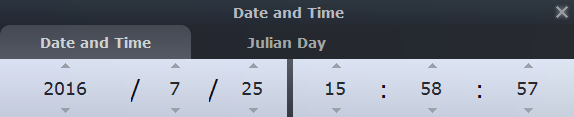
\includegraphics[width=0.75\textwidth]{date_and_time_dialog.png}
\caption{Date and Time dialog}
\label{fig:gui:date}
\end{figure}

In addition to the time rate control buttons on the main toolbar, you
can use the date and time window (open with the \guibutton[0.35]{2}{btd_time.png} 
button or \key{F5}) to set the simulation time. The values
for year, month, day, hour, minutes and seconds may be modified by
typing new values, by clicking the up and down arrows above and below
the values, and by using the mouse wheel.

The other tab in this window allows you to see or set
\indexterm{Julian Day} and/or \indexterm[Julian Day!Modified]{Modified Julian Day} numbers
(see~\ref{sec:Concepts:JulianDay}).

\section{Setting Your Location}
\label{sec:gui:location}

\begin{figure}[htbp]
\centering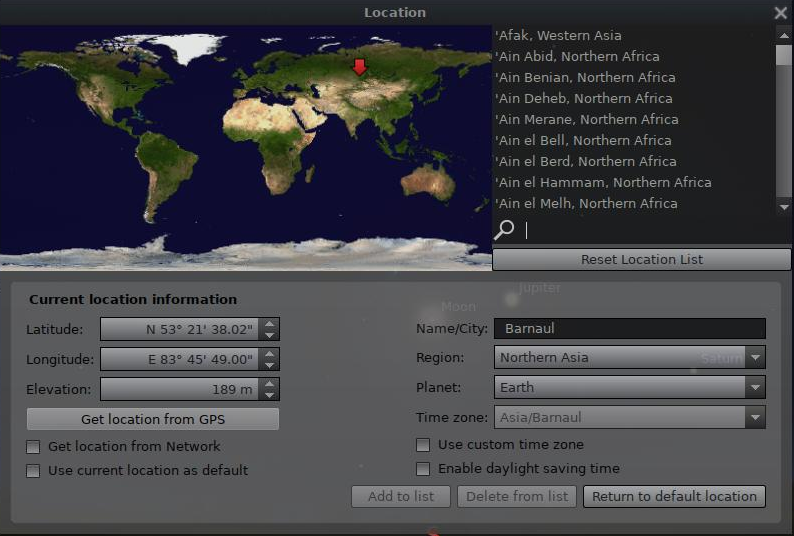
\includegraphics[width=0.85\textwidth]{location_dialog.png}
\caption{Location window}
\label{fig:gui:location}
\end{figure}

\noindent The positions of the stars in the sky is dependent on your location on
Earth (or other planet) as well as the time and date. For Stellarium to
show accurately what is (or will be/was) in the sky, you must tell it
where you are. You only need to do this once -- Stellarium can save your
location so you won't need to set it again until you move.

After installation\newFeature{0.13.1}, Stellarium uses an online service which tries to
find your approximate location based on the IP address you are
using. This seems very practical, but if you feel this causes privacy
issues, you may want to switch this feature off. You should also consider 
switching it off on a computer which does not move, to save network bandwidth.

To set your location more accurately, or if the lookup service fails,
press \key{F6} to open the location window (Fig.~\ref{fig:gui:location}). 
There are a few ways you can set your location:

\begin{enumerate}
\item Just click on the map.
\item Search for a city where you live using the search edit box at
  the top right of the window, and select the right city from the
  list.
\item Click on the map to filter the list of cities in the vicinity of
  your click, then choose from the shortlist.
\item Enter a new location using the longitude, latitude and other
  data.
\item Click on \menu{Get Location from GPS} if you have a GPS
  receiver. \newFeature{0.16/0.18.1} You activate a periodic request
  for GPS fixes. After a few seconds, the button should change color
  and give a textual feedback. Green indicates a good position, yellow
  indicates a 2D-fix only, which means altitudes are not
  available. (Leave the GPS device running for a few minutes and/or
  search a place with better sky view.) You could leave it running if
  you are operating a fast-moving observatory platform, but rather
  switch it off when you see a good fix, so that other programs can
  use the serial GPS connection.  Red signals an error, and further
  positions are not retrieved but the button is reset. You may press
  the button again to start over.

  Sometimes you have to try several times or let it run for a while to get a
  green button indicating a valid 3D fix including altitude.
  See section~\ref{sec:ExtraData:GPS} for configuration details.
\end{enumerate}

\noindent If you want to use the current location permanently, click on the
``use as default'' checkbox, disable ``Get location from Network'',
and close the location window.

Two settings may influence the landscape when changing locations:
\begin{description}
\item[Auto select landscapes] When changing the planet, 
a fitting landscape panorama will be shown when available. 
Also, \newFeature{23.2} when clicking on the earth map, 
a zero-altitude landscape is displayed in the approximate color of that location (taken from the map).
\item[Auto-enable atmosphere] When changing planet during
  location change, the atmosphere will be switched as required.
\end{description}

\subsection{Time Zones}
\label{sec:gui:location:timezones}
Locations in Stellarium's location database include their respective
time zone.\newFeature{0.15.1/0.19.0} When you click on a location in
the list, the time should be shown in the respective time zone.  If
daylight time rules exist and you have selected ``Enable daylight
saving time'', also this abomination of modern civilisation is respected. Most
users will require to have this setting active.

When you select ``Use custom time zone'', you can select other time zones.
Those that start with UTC have no daylight time rules.

Time zones were introduced in the 19th century, originally for
purposes of railway traffic synchronization. The first such action was
taken in 1847, and therefore Stellarium by default will present Local
Mean Solar Time (LMST) for dates before 1847, and ignore all
configured time zones unless you deliberately activate ``Use custom
time zone''. The history of time zones and their rules is very
complicated, though, and Stellarium should not be expected to find the
exact date when time zone use was introduced at a certain location or
country. Just be sure to use LMST when replaying historical
observations before the 20th century.

For even earlier observations, you can also set Local True Solar Time
(LTST), which is the time given by sundials. Here, 12 o'clock is the
time when the sun transits the meridian, strictly, daily. The
difference between LMST and LTST is called \emph{equation of time}. 
See section~\ref{sec:plugins:EquationOfTime} for more information.

When you click on the map to set your location, Stellarium has
currently no way to guess the timezone of the coordinate pair. In this
case, Local Mean Solar Time is presented, which only depends on
longitude and was the ``normal'' time before the development of time
zones. Either select a city from the list or manually select a time
zone.

\subsection{Geographical Regions}
\label{sec:gui:location:geographicalregions}

The world is split into political entities called ``countries''. \newFeature{0.21.2} 
Humans have an unappealing tendency of fighting over the question to which 
country some territories should be counted. Stellarium is an astronomy 
program which labels coordinates of locations like cities with a name. 
Earlier editions of Stellarium used countries as further superordinate 
entities to locations for identification purposes. In consequence to much 
unnecessary and unfriendly discussion we decided to completely drop the 
petty-minded assignment of political country names to locations in favour 
of geographical regions. There is only one known habitable planet, one 
humankind, and one sky. Stellarium users should overcome borders! 

For the ``region'' classification of sky cultures we use the same regions (see \ref{sec:skycultures:region}), 
and we follow the UN~M49 geoscheme\footnote{https://unstats.un.org/unsd/methodology/m49/} with extensions for other planets.

\subsection{Observers}
\label{sec:gui:location:observers}

In the list of Planets you can find entries called \emph{Solar System Observer}, \emph{Jupiter Observer} and 
similar for each major planet that has moons: Earth, Mars, Jupiter, Saturn, Uranus, and Neptune. 
These are specialized locations. When switching to them, you will find yourself looking 
onto the respective observed object (Sun, Jupiter, \ldots) from somewhat above the plane of the Solar system. 
By pressing \key{\Alt+\arrowkeyleft}/\key{\Alt+\arrowkeyright} you can rotate around a vertical axis through the observed object.
Likewise, by pressing \key{\Alt+\arrowkeyup}/\key{\Alt+\arrowkeydown} you can change the latitude of observation. Finally, 
with \key{\Alt+Home}/\key{\Alt+End} you can change the distance from the observed object. 


\section{The Configuration Window}
\label{sec:gui:configuration}

The configuration window contains general program settings, and many
other settings which do not concern specific display options. Press
the tool button \guibutton[0.35]{2}{btd_config.png} or \key{F2} to open.


\subsection{The Main Tab}
\label{sec:gui:configuration:main}


\begin{figure}[htbp]
\centering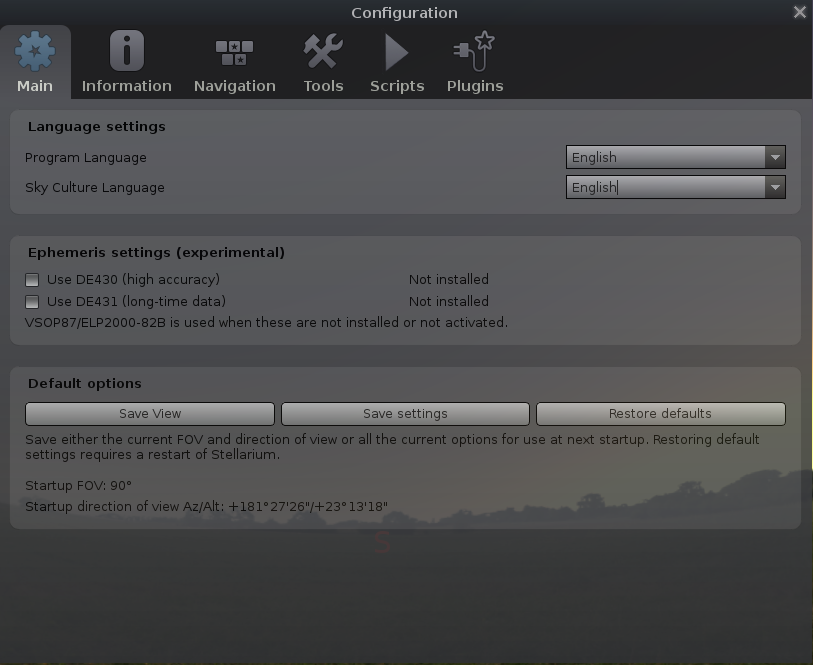
\includegraphics[width=0.75\textwidth]{config_dialog_main_tab.png}
\caption{Configuration Window: Main Tab}
\label{fig:gui:configuration:main}
\end{figure}

The Main tab in the configuration window (Fig.~\ref{fig:gui:configuration:main}) provides controls for
changing separately the program and sky culture languages.

The next setting group allows to enable using DE430/DE431 and DE440/DE441 ephemeris files. 
These files have to be installed separately. Most users do not require this. 
See section~\ref{sec:ExtraData:ephemerides} if you are interested.

The tab also provides the buttons for saving the current view direction as default 
for the next startup, and for saving the program configuration. 
Most display settings have to be explicitly stored to make a setting change permanent.

\subsection{The Information Tab}
\label{sec:gui:configuration:info}

\begin{figure}[htbp]
\centering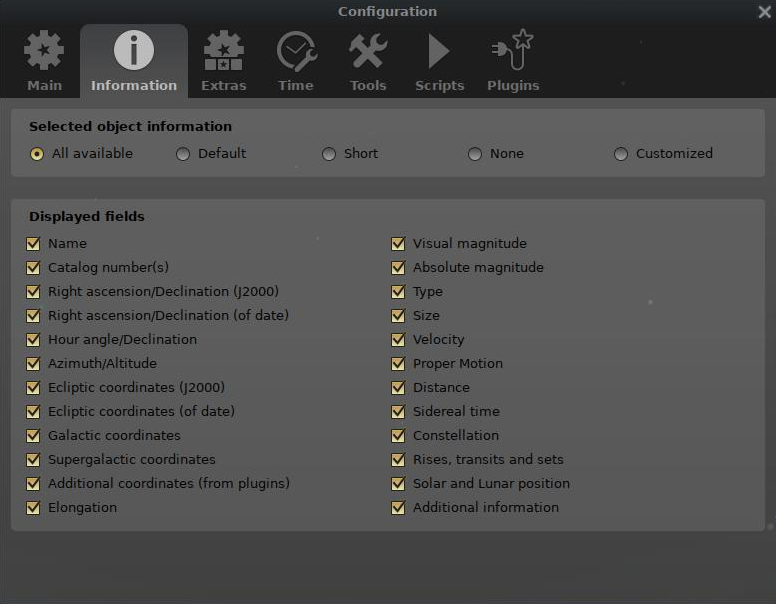
\includegraphics[width=0.75\textwidth]{config_dialog_info_tab.png}
\caption{Configuration Window: Information Tab}
\label{fig:gui:configuration:info}
\end{figure}

The Information tab (Fig.~\ref{fig:gui:configuration:info}) allows you to set the type and amount of information
displayed about a selected object.
\begin{itemize}
\item Ticking or unticking the relevant boxes will control this.
\item The information displays in various colors depending on the type and
level of the stored data
\end{itemize}

\subsection{The Extras Tab}
\label{sec:gui:configuration:extras}

\begin{figure}[htbp]
\centering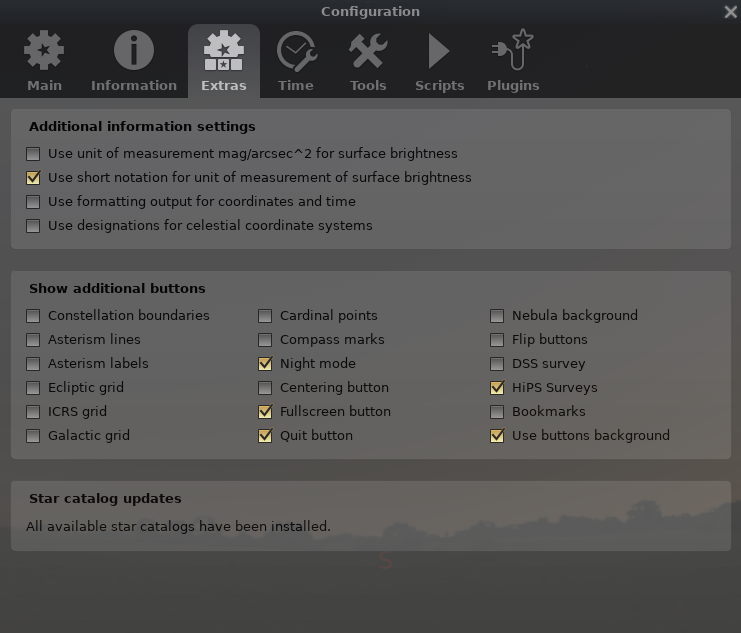
\includegraphics[width=0.75\textwidth]{config_dialog_extras_tab.png}
\caption{Configuration Window: Extras Tab}
\label{fig:gui:configuration:extras}
\end{figure}

The Extras tab (Fig.~\ref{fig:gui:configuration:extras}) allows you to
customize information displayed about a selected object, download more
star catalogs and also allows to hide or show additional buttons in
the lower button bar. 
\subsubsection{Customization of information displays}
The information display can be tweaked a bit with the options found in the GUI section ``Additional information settings''.

\subsubsection{Customization of button visibility on bottom toolbar}
If your screen is too narrow to show all buttons
or you simply don't need them because you prefer the keyboard shortcuts,
you can choose your optimal setup. The selection of buttons is stored immediately. 
\begin{description}
\item[Constellation boundaries] You can toggle display of constellation boundaries with this button.
\item[Asterism lines] You can toggle display of asterism lines with this button.
\item[Asterism labels] You can toggle display of asterism labels with this button.
\item[Ecliptic grid] You can toggle display of ecliptic coordinate grid with this button.
\item[ICRS grid] You can toggle display of the International Coordinate Reference System (equatorial J2000 coordinate grid) with this button.
\item[galactic grid] You can toggle display of galactic coordinate grid with this button.
\item[Cardinal points] You can toggle display of the ``Cardinal points'' button.
\item[Compass marks] You can toggle display of the ``Compass marks'' button.
\item[Night mode] You can toggle display of the nightmode button.
\item[Centering button] You can toggle display of the ``Center on selected object'' button.
\item[Fullscreen button] You can toggle display of the fullscreen button.
\item[Quit button] You can toggle display of the button to quit Stellarium.
\item[Nebula background] You can toggle display of DSO photographs with this button.
\item[Flip buttons] When enabled, two buttons will be added to
  the main tool bar which allow the main view to be mirrored in the
  vertical and horizontal directions. This is useful when observing
  through telecopes which may cause the image to be mirrored.
\item[DSS survey] You can toggle display of Digitized Sky Survey with this button (see section~\ref{sec:TOAST}).
\item[HiPS Surveys] You can toggle display of Hierarchical Progressive Surveys with this button (see section \ref{sec:gui:view:surveys}).
\item[Bookmarks] You can enable display of Bookmarks (Observing Lists) dialog with this button.
\item[Use buttons background] Applies a gray background under the buttons on the bottom bar.
\end{description}

\subsubsection{Download more star catalogs}
Stellarium comes with enough stars for casual stargazing with the
unaided eye or binoculars. If you have a telescope and want to see
more stars, here you can download more catalogs. (See Appendix~\ref{ch:Catalogues})

\subsection{The Time Tab}
\label{sec:gui:configuration:time}

\begin{figure}[htbp]
\centering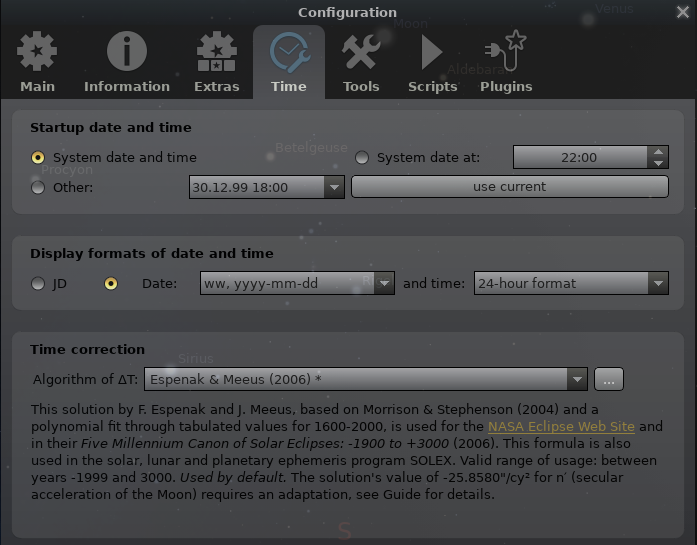
\includegraphics[width=0.75\textwidth]{config_dialog_time_tab.png}
\caption{Configuration Window: Time Tab}
\label{fig:gui:configuration:time}
\end{figure}

The Time tab (Fig.~\ref{fig:gui:configuration:time}) allows to specify what simulation time should be used
when the program starts:

\begin{description}
\item[System date and time] Stellarium will start with
  the simulation time equal to the operating system clock.
\item[System date at] Stellarium will start with the
  same date as the operating system clock, but the time will be fixed at
  the specified value. This is a useful setting for those people who use
  Stellarium during the day to plan observing sessions for the upcoming
  evening.
\item[Other] some fixed time can be chosen which will
  be used every time Stellarium starts.
\end{description}

\noindent The middle field allows specify display formats for date and time on bottom toolbar:
\begin{description}
\item[JD] Stellarium will display Julian Days (JD).
\item[Date and time] Stellarium will display date and time in selected format.
\end{description}

\noindent The lowest field allows selection of the correction model for the time
correction $\Delta T$ (see section~\ref{sec:Concepts:DeltaT}). Default
is ``Modified Espenak and Meeus (2006)''. Please use other values only if you
know what you are doing.

\subsection{The Tools Tab}
\label{sec:gui:configuration:tools}

\begin{figure}[htbp]
\centering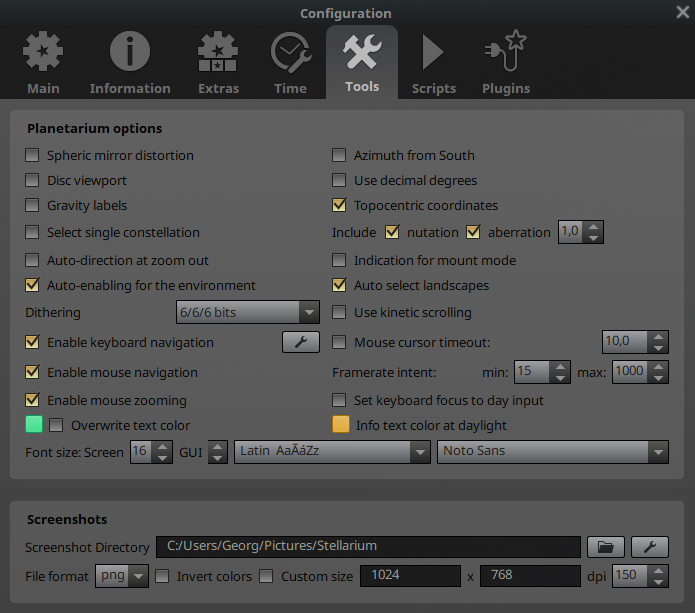
\includegraphics[width=0.75\textwidth]{config_dialog_tools_tab.png}
\caption{Configuration Window: Tools Tab}
\label{fig:gui:configuration:tools}
\end{figure}

The Tools tab (Fig.~\ref{fig:gui:configuration:tools}) contains planetarium options 
(like enabling/disabling of keyboard shortcuts for panning and zooming the main view) 
and options for screenshots.

\begin{description}
\item[Spheric mirror distortion] This option pre-warps the main view
  such that it may be projected onto a spherical mirror using a
  projector. The resulting image will be reflected up from the spherical
  mirror in such a way that it may shine onto a small planetarium
  dome (or even just the ceiling of your dining room), making a cheap planetarium projection system.
\item[Disc viewport] This option masks the main view
  producing the effect of a telescope eyepiece. It is also useful when
  projecting Stellarium's output with a fish-eye lens planetarium
  projector.
\item[Gravity labels] This option makes labels of objects in the
  main view align with the nearest horizon. This means that labels
  projected onto a dome are always aligned properly.
\item[Select single constellation] When active, clicking on a star
  that is member in the constellation lines will make the
  constellation stand out. See section~\ref{sec:starlore:singleConstellations} for details.
\item[Dithering] options to allow select better simulation of sky on different hardware.
\item[Auto zoom out returns to initial direction of view] When enabled,
  this option changes the behavior of the zoom out key
  \key{\textbackslash{}} so that it resets the initial direction of view in
  addition to the field of view.
\item[Enable keyboard navigation]
\item[Enable mouse navigation]
\item[Enable mouse zooming]
\item[Overwrite text color] --- enabling this option\newFeature{0.20.2} will ignore the 
  color settings for each celestial object and enable one color for text on the info panel 
  for all celestial objects. By default Stellarium uses white color for this option, 
  but you may re-define it through a color chooser\newFeature{0.20.3}.
\item[Set keyboard focus to day input] --- you may use this option to force setting the 
  keyboard focus on the day input field in the Date and Time dialog. 
  
  Important note: the focus in the sky will be lost when you open the 
  Date and Time dialog after enabling this option.
\item[Azimuth from South] Some users may be used to counting azimuth
  from south.
\item[Use decimal degrees] You can toggle usage of decimal degree format for coordinates.
\item[Topocentric coordinates] If you require planetocentric coordinates, you may switch this off. 
  Usually it should be enabled. (See~\ref{sec:Concepts:Parallax:Topocentric})
\item[Include nutation] Compute the slight wobble of earth's
  axis. This feature is active only about 500 years around J2000.0.
\item[Include aberration] Add effect of annual \indexterm{aberration of light} to the object's position (see \ref{sec:Concepts:Aberration}). 
     Note: This also influences the displayed position in the J2000 frame!
	 For didactic purposes you can exaggerate the effect by up to $5\times$. 
\item[Indication for mount mode] You can activate the short display of a message when switching type of used mount.
\item[Edit keyboard shortcuts\ldots] See section~\ref{sec:gui:help:hotkeys}.
\item[Mouse cursor timeout] You can decide whether, and when, the
  mouse cursor should disappear from view when not moved.
\item[Info text color at daylight] --- this is a color chooser\newFeature{0.20.3} for defining the 
  text color for the info panel at daylight to increase the contrast of the text. 
  By default Stellarium use black color.
\item[Use kinetic scrolling]  Text fields in \newFeature{0.18.3} 
dialogs can either be moved on sidebar handles (with this switch
disabled) or by dragging the text itself (enabled), as it is known
from touch-enabled devices like smartphones. 
\end{description}

\paragraph{Framerate intent} \label{sec:gui:configuration:tools:fps} The pace of screen updates (frames per second, FPS) depends on several factors: 
CPU speed, graphics card speed, screen size, number of displayed objects and grids, etc. 
As is common for interactive programs, the main program thread runs on a single core also on a multicore system. 
For running Stellarium, a CPU with few but fast cores will appear faster in total than a multicore system at slower CPU cycles.  
High-end systems may deliver needlessly high framerates, at cost of energy consumption.
The maximum FPS setting limits the frame rate when Stellarium is interactively operated 
(zoomed, panned, settings switched, etc.) 
After a few seconds, when Stellarium is not interactively operated, it falls back to a minimum FPS setting to conserve energy. 
Of course, when the system cannot even reach this FPS, the factual FPS will be lower and the system may be overloaded.
Keep in mind that the mimimum setting also applies to running scripts (non-interactively).

\paragraph{Font size and font selection} \newFeature{0.18.3} You can change the font sizes for on-screen
text and GUI dialogs separately.  For some purposes like presentations
it may be helpful to enlarge screen font size while keeping GUI font
regular, or vice versa.  It also depends on your screen size whether
all the object info fits on screen. This may also depend on the
writing system and installed font. If you are using a non-Western
character system and the default font looks bad, you can select
another system font. For this, edit \file{config.ini} (see
chapter~\ref{sec:Directories}): locate the \texttt{[gui]} section and
set the key \texttt{flag\_font\_selection=true}. On next start of
Stellarium, you will find two elements for font selection: one allows
you to pre-select a writing system, the other will then allow
selection of a font installed in your system that includes the
characters used in the selected writing system. When you have found
the best font, store your settings on the Main tab (see
section~\ref{sec:gui:configuration:main}) and you may edit
\file{config.ini} again to disable the font selection switches.

\paragraph{Screenshots} You can set the directory where screenshots
will be stored, and \newFeature{0.18.1} also whether you want
screenshots sized like Stellarium's window or some other, likely
larger size. The maximum possible size depends on your
hardware. $4096\times4096$ should be possible on most PCs, others may
even create $16384\times16384$ images. The vertical field of view will be the same as in the current view.

You can also set \newFeature{0.19.0} the file format. The exact selection depends on
platform and version of the underlying Qt framework. Notable formats are PNG (lossless), JPG (lossy),
JPEG (higher quality JPG), BMP (Windows Bitmap), WEBP, TIF (LZW compressed), TIFF (uncompressed),
PBM, PGM, PPM, XBM, XPM, and ICO (thumbnails).

Some printing workflows require particular DPI (dots per inch)
settings stored in the screenshots. \newFeature{0.22.0} You can
configure DPI which will be stored in the image metadata. The intended
print size in \mm\ is shown in the tooltip of the dpi spinner.

\subsection{The Scripts Tab}
\label{sec:gui:configuration:scripts}

\begin{figure}[htbp]
\centering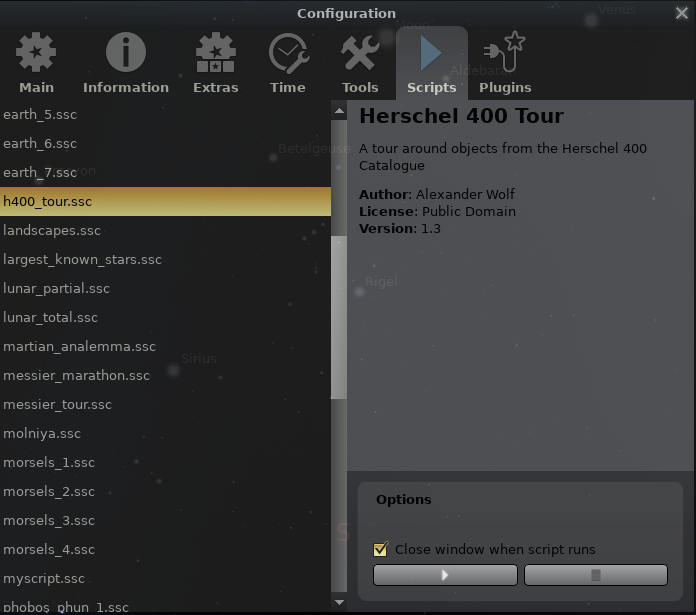
\includegraphics[width=0.75\textwidth]{config_dialog_scripts_tab.png}
\caption{Configuration Window: Scripts Tab}
\label{fig:gui:configuration:scripts}
\end{figure}

The Scripts tab (Fig.~\ref{fig:gui:configuration:scripts}) allows the
selection of pre-assembled scripts bundled with Stellarium that can be
run (See chapter~\ref{ch:scripting} for an introduction to the
scripting capabilities and language). This list can be expanded with
your own scripts as required. See
section~\ref{sec:FilesAndDirectories:DirectoryStructure} where to
store your own scripts.

When a script is selected it can be run by pressing the arrow button
and stopped with the stop button. With some scripts the stop button is
inhibited until the script is finished. %% TODO: EXPLAIN HOW?

Scripts that use sound or embedded videos will need a version of
Stellarium configured at compile time with multimedia support
enabled. It must be pointed out here that sound or video codecs
available depends on the sound and video capabilities of you computer
platform and may not work.


\subsection{The Plugins Tab}
\label{sec:gui:configuration:plugins}

\begin{figure}[htbp]
\centering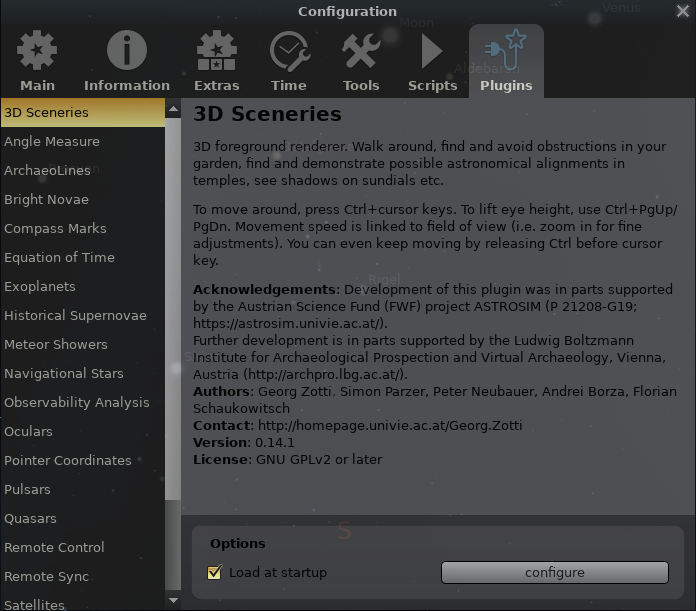
\includegraphics[width=0.75\textwidth]{config_dialog_plugins_tab.png}
\caption{Configuration Window: Plugins Tab}
\label{fig:gui:configuration:plugins}
\end{figure}


Plugins (see chapter~\ref{ch:Plugins} for an introduction) can be
enabled here (Fig.~\ref{fig:gui:configuration:plugins}) to be loaded the next time
you start Stellarium. When loaded, many plugins allow additional configuration
which is available by pressing the \menu{configure} button on this tab.


\section{The View Settings Window}
\label{sec:gui:view}

The View settings window controls many display features of Stellarium
which are not available via the main toolbar.

\subsection{The Sky Tab}
\label{sec:gui:view:sky}

\begin{figure}[htbp]
\centering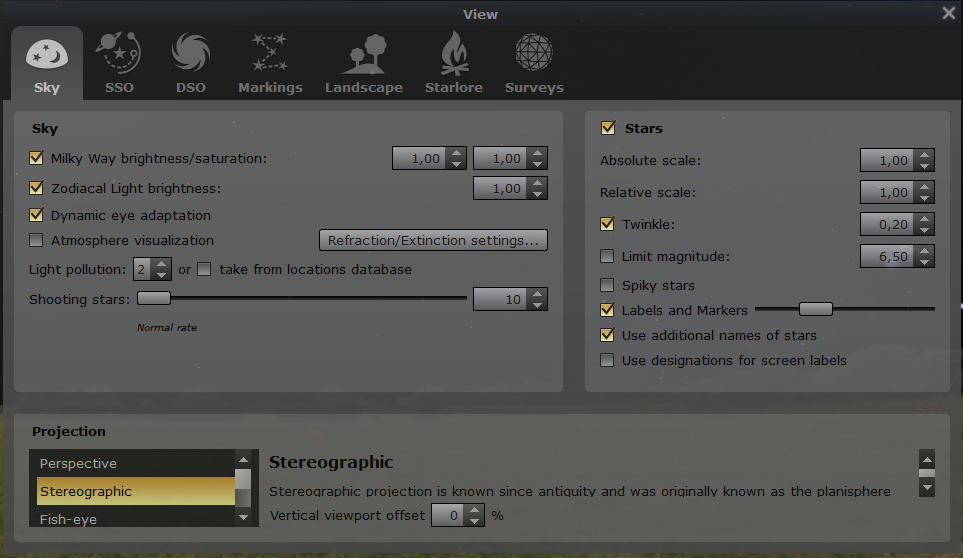
\includegraphics[width=0.75\textwidth]{view_dialog_sky_tab.png}
\caption{View Settings Window: Sky Tab}
\label{fig:gui:view:sky}
\end{figure}

The Sky tab of the View window (Fig.~\ref{fig:gui:view:sky}) contains settings
for changing the general appearance of the main sky view and projections. Some highlights of sky field:
\begin{description}
\item[Dynamic eye adaptation] When enabled this feature reduces the
  brightness of faint objects when a bright object is in the field of
  view. This simulates how the eye can be dazzled by a bright object
  such as the moon, making it harder to see faint stars and galaxies.
\begin{samepage} % If the list of options is page-broken from the beginning of the "Light pollution" item, it becomes hard to orient in the text due to starting a page with a nested list.
\item[Light pollution] In urban and suburban areas, the sky is
  brightened by terrestrial light pollution reflected in the atmosphere.
  Stellarium simulates light pollution and lets the user configure how bright
  the night sky is.
  There are several ways to set it up:
  \begin{description}
    \item[Automatic from locations database] option makes Stellarium find sky
      brightness from its locations database and simulate light pollution
      without any further user input.
    \item[Manual] mode lets the user choose the amount of light pollution by
      moving a slider. To make it easier to orient in the resulting amount of
      light pollution, a tooltip will show the classification of the sky
      according to the \emph{Bortle Dark Sky Scale} (See Appendix~\ref{ch:BortleScale}
      for more information), as well as the naked-eye limiting magnitude.
    \item[Manual from SQM] mode lets one enter the reading of a \emph{Sky Quality Meter}.
      Stellarium can accept it in several units: physical ($\mathrm{cd/m^2}$,
      $\mathrm{mcd/m^2}$, $\mathrm{\mu cd/m^2}$) as well as astronomical,
      $\mathrm{mag/arcsec^2}$. To enter a value, first choose the unit, and
      then type the number into the spinbox.
  \end{description}
\end{samepage}
\item[Solar altitude for Twilight Finder] You can configure \newFeature{0.21.2} 
shortcut keys to go to the time when the sun reaches this altitude below the 
mathematical horizon. See section~\ref{sec:gui:help:hotkeys:example}.
\item[Shooting stars] Stellarium has a simple meteor simulation
  option. This setting controls how many shooting stars will be shown.
  Note that shooting stars are only visible when the time rate is 1, and
  might not be visible at some times of the day. Meteor showers can be
  simulated using a dedicated plugin (see section~\ref{sec:plugins:MeteorShowers}).
\end{description}

\noindent Some highlights of the stars field:
\begin{description}
\item[Absolute scale] is the size of stars as rendered by
  Stellarium. If you increase this value, all stars will appear larger
  than before.
\item[Relative scale] determines the difference in size of bright
  stars compared to faint stars. Values higher than 1.00 will make the
  brightest stars appear much larger than they do in the sky. This is
  useful for creating star charts, or when learning the basic
  constellations.
\item[Twinkle] controls how much the stars twinkle when atmosphere is
  enabled (\indexterm{scintillation}, see section~\ref{sec:phenomena:Scintillation}). 
  Since v0.15.0, the twinkling is reduced in higher altitudes,
  where the star light passes the atmosphere in a steeper angle and is
  less distorted.
\item[Limit magnitude] Inhibits automatic addition of fainter stars
  when zooming in. This may be helpful if you are interested in naked
  eye stars only.
\item[Labels and markers] you can independently change the amount of
  labels displayed for stars. The further to the
  right the sliders are set, the more labels you will see. Note that
  more labels will also appear as you zoom in.
\item[Use designations for screen labels] --- when this option is
  enabled you will see in the sky (on-screen labels) only scientific
  designations (catalog numbers) of the stars instead of their common
  names. To customize\newFeature{0.21.3} the on-screen labels we
  added 3 additional options\footnote{These options are only used if the 
  star does not have Bayer/Flamsted designations.}
 --- \textbf{Dbl. stars}, \textbf{Var. stars} and \textbf{HIP} --- which will show, 
  in this sequence of preference, the first available occurrence of 
  the traditional designations of double stars, 
  variable stars or HIP numbers, respectively. 
\end{description}

\subsubsection{The Projections field}
\label{sec:gui:view:sky:projections}

Selecting items in this list changes the
  projection method which Stellarium uses to draw the sky~\citep{Snyder:MapProjections}. Options are:

\begin{description}
  \item[Perspective] Perspective projection maps the horizon and other
    great circles like equator, ecliptic, hour lines, etc. into
    straight lines. The maximum field of view is 150\degree. The
    mathematical name for this projection method is \emph{gnomonic
      projection}.
  \item[Stereographic] Stereographic projection has been known since
    antiquity and was originally known as the planisphere
    projection. It preserves the angles at which curves cross each
    other but it does not preserve area. Else it is similar to
    fish-eye projection mode. The maximum field of view in this mode
    is 235\degree.
  \item[Fish-Eye] Stellarium draws the sky using \emph{azimuthal
    equidistant projection}. In fish-eye projection, straight lines
    become curves when they appear a large angular distance from the
    center of the field of view (like the distortions seen with very
    wide angle camera lenses). This is more pronounced as the user zooms
    out. The maximum field of view in this mode is 180\degree.
  \item[Orthographic] Orthographic projection is related to
    perspective projection, but the \emph{point of perspective} is set
    to an infinite distance. The maximum field of view is 180\degree.
  \item[Equal Area] The full name of this projection method is
    \emph{Lambert azimuthal equal-area projection}. It preserves the
    area but not the angle. The maximum field of view is 360\degree.
  \item[Hammer-Aitoff] The Hammer projection is an equal-area map
    projection, described by \name[Ernst von]{Hammer} (1858--1925) in 1892 and directly inspired
    by the Aitoff projection. The maximum field of view in this mode is
    360\degree.
  \item[Sinusoidal] The sinusoidal projection is a
    \emph{pseudocylindrical equal-area map projection}, sometimes
    called the Sanson--Flamsteed or the Mercator equal-area
    projection. Meridians are mapped to sine curves.
  \item[Mercator] Mercator projection is a cylindrical projection developed 
    by \name[Gerardus]{Mercator} (1512--1594)
    which preserves the angles between objects, and the scale around
    an object is the same in all directions. The poles are mapped to
    infinity.  The maximum field of view in this mode is 233\degree.
  \item[Miller cylindrical] The Miller cylindrical projection is a
    modified Mercator projection, proposed by \name[Osborn Maitland]{Miller}
    (1897--1979) in 1942. The poles are no longer mapped to
    infinity.
  \item[Cylinder] The full name of this simple projection mode is
    \emph{cylindrical equidistant projection} or \emph{Plate
      Carr\'ee}. The maximum field of view in this mode is 233\degree.
\end{description}

\noindent Two more settings allow finetuning:
\begin{description}
\item[Vertical viewport offset] If you have a wide screen or like wide-angle views,
you may feel that too much of screen space lies below the horizon. This setting can shift the view up or down.
\item[Custom FoV limit] Some projections allow very wide views, like 180°
which covers a complete \newFeature{0.21.2} celestial hemisphere (e.g.\ the entire skydome)
or even more. In some cases like if you are running a planetarium, you may want
to limit the vertical field of view so that you won't ever zoom out too far.
\end{description}

\subsubsection{Atmosphere settings}
\label{sec:gui:view:sky:atmosphere}

An auxiliary dialog opens when you select \guibutton[1.0]{0.75}{uibtSettings.png}
and contains detail settings for the atmosphere. Here
you can choose visual model of atmosphere, set atmospheric pressure and temperature which influence
refraction (see section~\ref{sec:phenomena:Refraction}) and the
opacity factor $k_v$ for extinction, \emph{magnitude loss per airmass} 
(see section~\ref{sec:phenomena:Extinction}).

There are two visual models for the atmosphere available:
\begin{description}
  \item[Preetham] This is the legacy model (see section~\ref{sec:skylight:Preetham}), fallback for the cases
    when the other one doesn't work.
  \item[ShowMySky] This model is the more realistic visual model of
    the atmosphere colors (see section~\ref{sec:skylight:ShowMySky}). It
    relies on a precomputed dataset that can be chosen in the user
    interface after the \program{ShowMySky} model is enabled.
\end{description}

\subsection{The Solar System Objects (SSO) Tab}
\label{sec:gui:view:sso}

The Solar System Objects tab of the View window (Fig.~\ref{fig:gui:view:sso}) contains settings
for changing the general appearance of the view of Solar system objects. Some highlights:

\begin{figure}[htbp]
\centering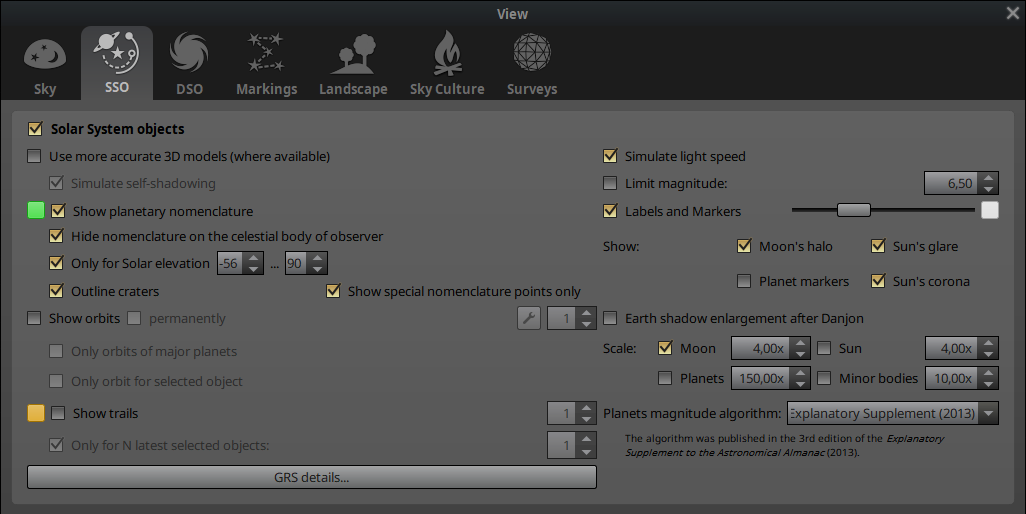
\includegraphics[width=0.75\textwidth]{view_dialog_sso_tab.png}
\caption{View Settings Window: SSO Tab}
\label{fig:gui:view:sso}
\end{figure}


\begin{description}
\item[Simulate light speed] will give more precise positions for planetary bodies which move
  rapidly against background stars (e.g. the moons of Jupiter).
\item[Scale] will increase the apparent size of the selected class of objects:
  \begin{description}
  \item[Moon] will increase the apparent size of the Moon
  in the sky, which can be nice for wide field of view shots.
  \item[Minor bodies] will increase the apparent size of minor
  bodies: planet satellites, all kinds of asteroids, and comets.  
  Forsome of these 3D models are available, which will be better
  discernible if enlarged.
  \item[Sun] will increase the apparent size of the Sun
    in the sky, which can be nice for didactic purposes or demonstrations.
  \item[Planets] will increase the apparent size of major planets.
  \end{description}
\item[Show orbits] adds a rendition of the orbit or trajectory of an SSO. 
For efficiency, orbits are not displayed when the object is not inside the screen, 
unless you set the ``permanently'' option. You can further fine-tune the selection 
and appearance (width and colors) of orbits with the additional settings. 
\item[Show trails] plots the apparent path of SSO among the stars as
  seen from the current planet.
\item[Show planetary nomenclature] displays positions and names of
  surface features officially named by the IAU (See
  Appendix~\ref{ch:Nomenclature}). When the sun is below the horizon
  at the location of the feature, the label is attenuated. Features like
  craters are best visible when they are illuminated by a low sun. 
  You can therefore limit the display\newFeature{1.2} to items along the
  \indexterm{terminator} (the border between light and dark on the surface).
\item[GRS details\ldots]: The Great Red Spot (GRS) is slowly
  drifting along Jupiter's System~II coordinate system. This button 
  opens a new dialog in which you can adjust the longitude (Jupiter system~II) 
  and annual drift rate of this feature at a particular epoch. To help you,
  another button in this dialog opens a website with relevant data.
  The central meridian data given
  \newFeature{0.21.0} in the object information on screen still shows
  System~II longitude.
\item[Labels and markers] you can independently change the amount of
  labels displayed for Solar system objects. The further to the
  right the sliders are set, the more labels you will see. Note that
  more labels will also appear as you zoom in.
\item[Planet magnitude algorithm] several ways to compute planet
  magnitudes have been made available from the literature. Data by
  Müller (1893) provide visual magnitudes. The other models provide
  instrumental (Johnson V) magnitudes.
\item[Earth shadow enlargement after Danjon] \newFeature{0.21.0}
  Earth's shadow is enlarged by the atmosphere. You can select whether
  the 2\% enlargement used by the Astronomical Almanac should be
  applied (default), or the formulation of \name{Danjon}
  (see section~\ref{sec:Eclipses:lunar}).
\end{description}

% Put these 3 on 1 page.
\begin{figure}[p]
\centering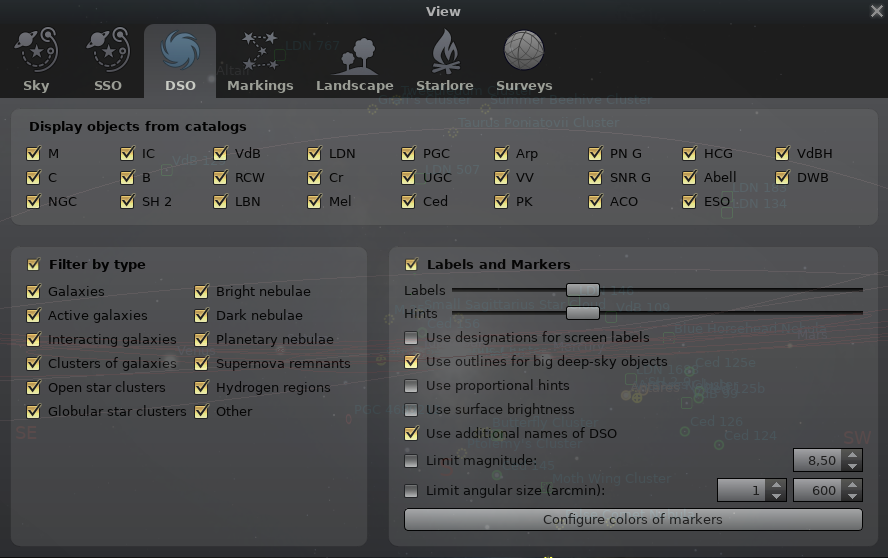
\includegraphics[width=0.75\textwidth]{view_dialog_dso_tab.png}
\caption{View Settings Window: DSO Tab}
\label{fig:gui:view:dso}
\end{figure}

\begin{figure}[p]
\centering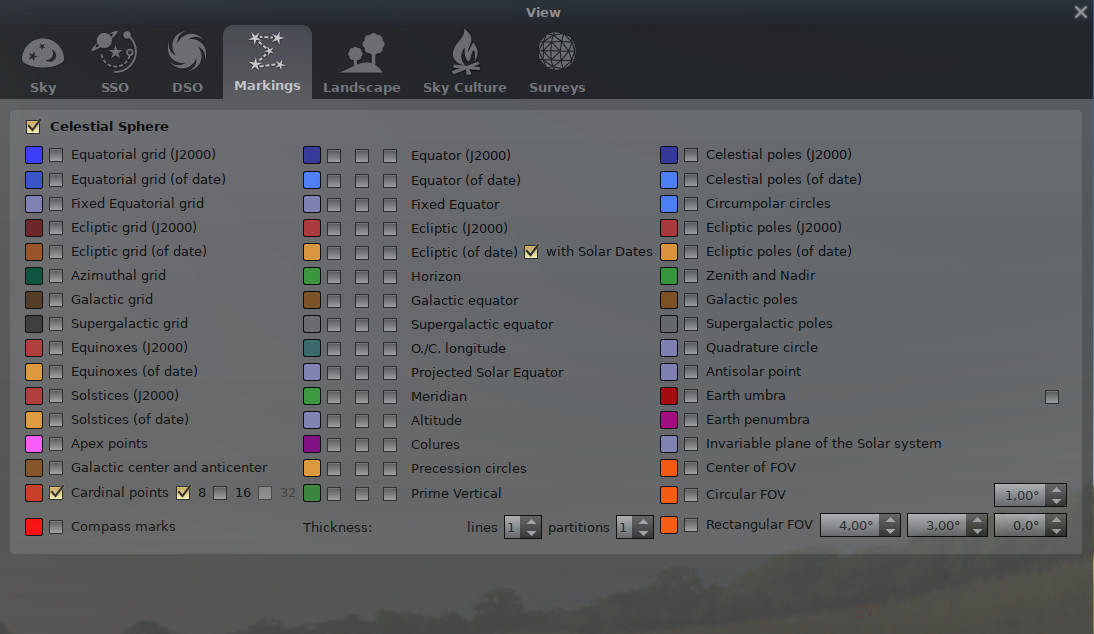
\includegraphics[width=0.75\textwidth]{view_dialog_markings_tab.jpg}
\caption{View Settings Window: Markings Tab}
\label{fig:gui:view:markings}
\end{figure}

\begin{figure}[p]
\centering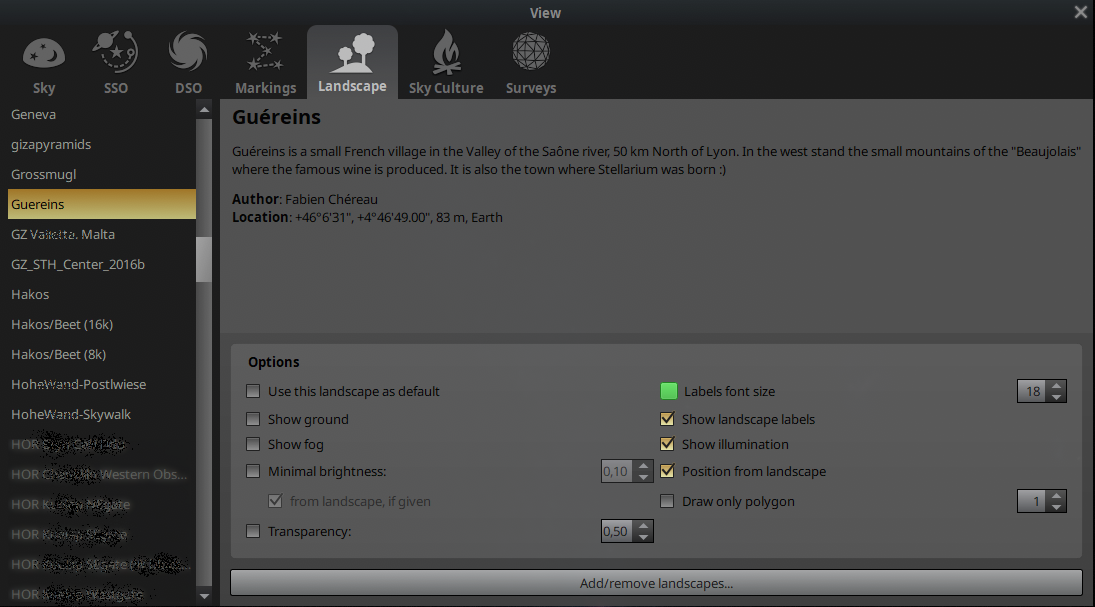
\includegraphics[width=0.75\textwidth]{view_dialog_landscape_tab.png}
\caption{View Settings Window: Landscape Tab}
\label{fig:gui:view:landscape}
\end{figure}

\subsection{The Deep-Sky Objects (DSO) Tab}
\label{sec:gui:view:dso}

\indexterm{Deep-sky objects} or DSO are extended objects which are
external to the solar system, and are not point sources like stars.
DSO include galaxies, planetary nebulae and star clusters. These
objects may or may not have images associated with them. Stellarium
comes with a catalog of over 90,000 extended objects containing
the combined data from many catalogs, with 500+ images.  

The DSO tab (Fig.~\ref{fig:gui:view:dso}) allows you to specify which 
catalogs or which object types you are interested in. This selection 
will also be respected in other parts of the program, 
most notably Search (section~\ref{sec:gui:search}) and 
AstroCalc/WUT (section~\ref{sec:gui:AstroCalc:WUT}) 
will not find objects from catalogs which you have not selected here. 

See chapter~\ref{ch:DSO} for details about the catalog, 
and how to extend it with your own photographs.


\subsection{The Markings Tab}
\label{sec:gui:view:markings}

\noindent The Markings tab of the View window
(Fig.~\ref{fig:gui:view:markings}) controls plotting various grids and
lines on the celestial sphere. Colors for grids, lines and points can be
adjusted by clicking on the corresponding colored square.  The central
column governs lines like equator, ecliptic, meridian etc., where each
can optionally be fine-tuned to \newFeature{0.20.0} show partition
marks and labels. Color settings are stored immediately, all other
flags need explicit saving of the settings (see section
\ref{sec:gui:configuration:main}).

\subsection{The Landscape Tab}
\label{sec:gui:view:landscape}

The Landscape tab of the View window
(Fig.~\ref{fig:gui:view:landscape}) controls the landscape graphics
(the horizon which surrounds you). To change the landscape graphics,
select a landscape from the list on the left side of the window. A
description of the landscape will be shown on the right.

Note that while a landscape  can include information about where the
landscape graphics were taken (planet, longitude, latitude and
altitude), this location does not have to be the same as the location
selected in the Location window, although you can set up Stellarium such
that selection of a new landscape will alter the location for you.

The controls at the bottom right of the window operate as follows:

\begin{description}
\item[Use this landscape as default] Selecting this option will save
  the landscape into the program configuration file so that the current
  landscape will be the one used when Stellarium starts.
\item[Show ground] This turns on and off landscape rendering (same
  as the button \guibutton{0.6}{bt_ground.png} in the main tool bar).
\item[Show fog] This turns on and off rendering of a band of
  fog/haze along the horizon, when available in this landscape.
\item[Show illumination] to reflect the ugly developments of our
  civilisation, landscapes can be configured with a layer of light
  pollution, e.g., streetlamps, bright windows, or the sky glow of a
  nearby city. This layer, if present, will be mixed in when it is
  dark enough.
\item[Show landscape labels] Landscapes can be configured with a
  gazetteer of interesting points, e.g., mountain peaks, which can be
  labeled with this option. Color and font size can also be configured.
\item[Position from landscape] When enabled, selecting a
  new landscape will automatically update the observer location.
  Use this if the landscape is not just decoration, but a true
  representation of a particular site you wish to visit in the simulation.
\item[Minimal brightness] Moonless night on very dark locations may appear too dark
  on your screen. You may want to configure some minimal brightness here.
  \begin{description}
\item[from landscape, if given] Landscape authors may decide to
  provide such a minimal brightness value in the \file{landscape.ini}
  file. 
  \end{description}
\item[Draw only polygon]\newFeature{0.20.2} If a polygonal horizon line has been
  defined for the landscape, only draw this with the given thickness.
\item[Transparency] Allow peeking below the horizon. \newFeature{23.3} Note that this may show graphical errors. 
\end{description}

\noindent Using the button \menu{Add/remove landscapes\ldots}, you can also
install new landscapes from ZIP files which you can download e.g.\
from the Stellarium
website\footnote{\url{https://stellarium.org/landscapes.html}}
or create yourself (see ch.~\ref{ch:landscapes} Landscapes), or remove
these custom landscapes.

Loading large landscapes may take several seconds. \newFeature{0.15.2}
If you like to switch rapidly between several landscapes and have enough memory, 
you can increase the default cache size to keep more landscapes loaded previously 
available in memory. Note that a large landscape can take up 200MB or more! 
See section \ref{sec:configini:landscape}.

\subsection{The Starlore Tab}
\label{sec:gui:view:starlore}


\begin{figure}[th]\centering
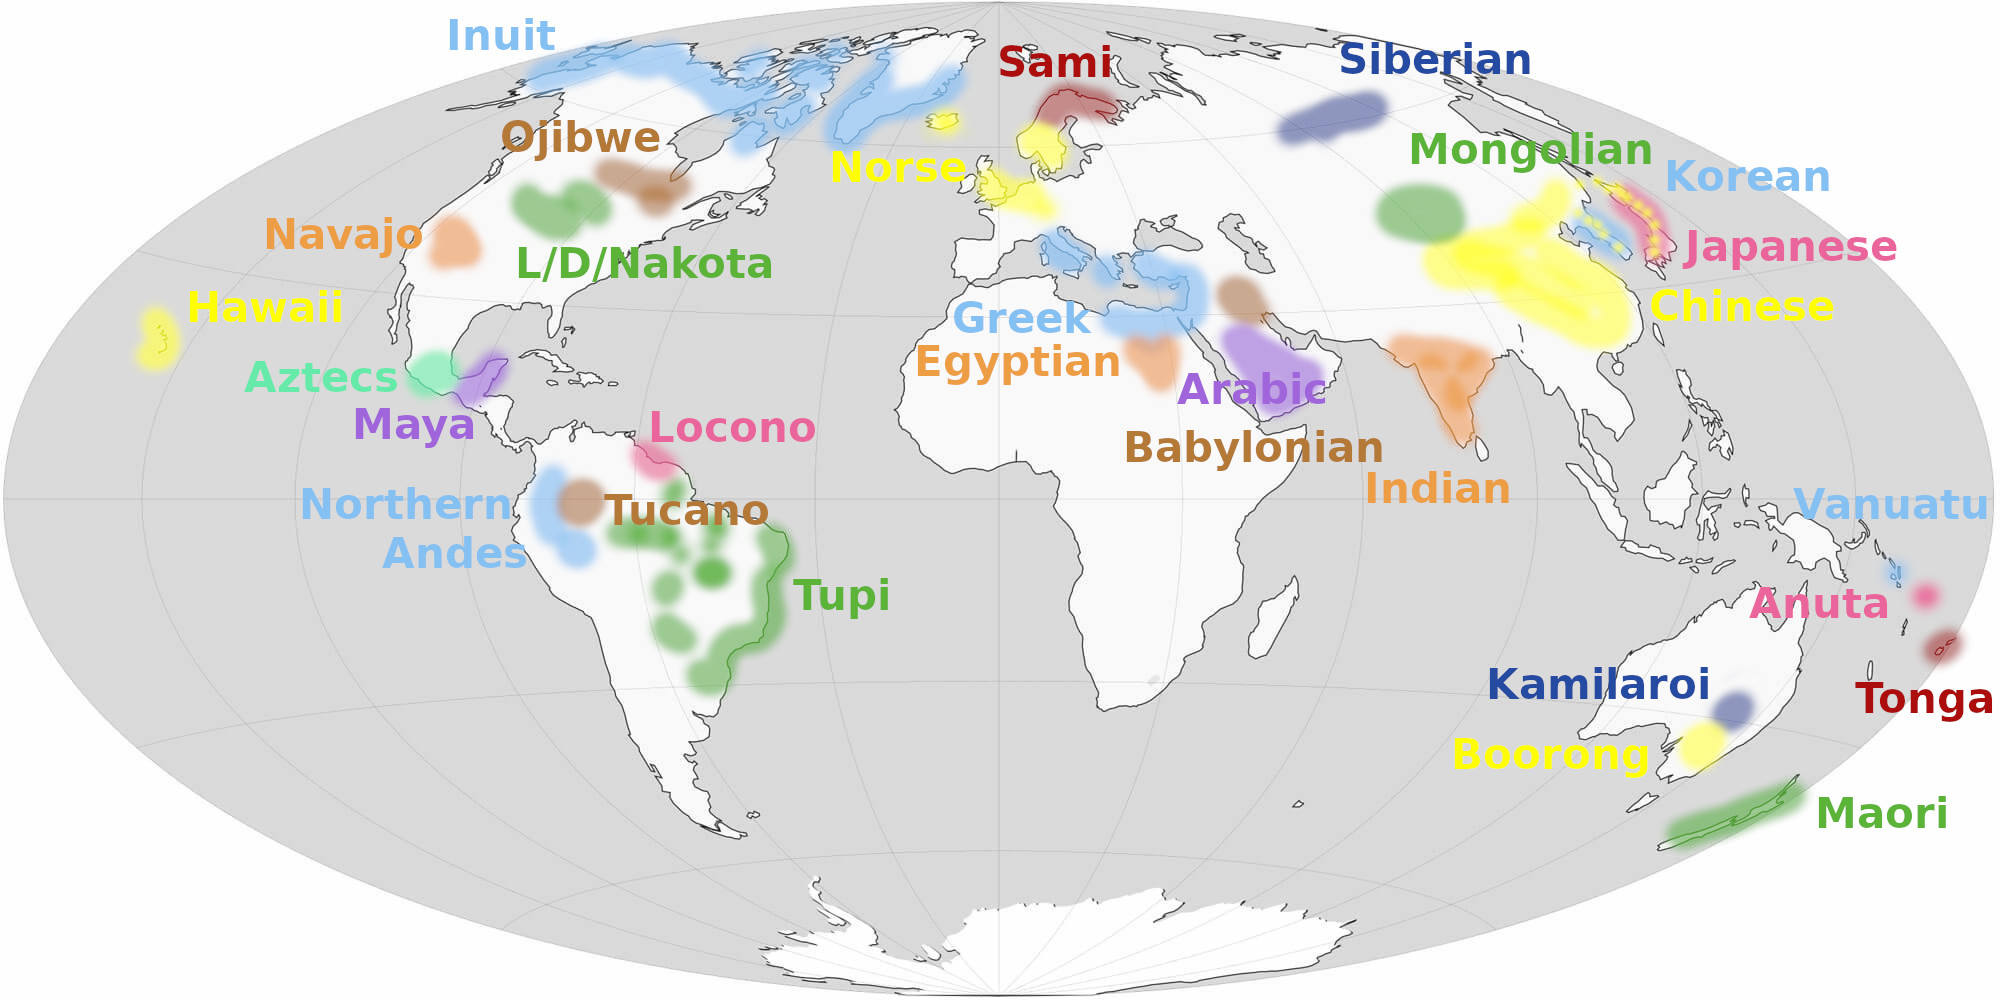
\includegraphics[width=\textwidth]{stellarium-skycultures-map.jpg}
\caption{World map showing Stellarium's built-in set of
  sky cultures. To avoid overcrowding, smaller European sky cultures
  which are mostly derivatives or relatives of the ``Modern'' sky culture are not
  shown. (Image: S. M. Hoffmann)}
\label{fig:skycultures}
\end{figure}

\noindent If you want to explore humankind's cultural history, you could also
switch to the viewpoint of other ancient or contemporary
people. Constellations are defined as patterns in the sky serving to
set calendar marks and to navigate while travelling on Earth. Which
patterns are seen depends on the natural environment and the cultural
habits of the people, i.e., the Inuit in the arctic area might have
seen an Elk where the Chinese have seen a huge spoon or dipper. There
cannot be any astrological influence from these patterns as they had
been seen differently and, thus, are a product of human's
imagination. So, pointing out these cultural differences might have an
educational function, too.

\noindent%
\colorbox{light-gray}{\fbox{\parbox[t]{0.975\linewidth}{
\paragraph{Caution} Some of our native peoples' constellations are contributed for noncommercial use only.
Please respect their heritage holders and check-out the CC licence
version in the description before you use sky cultures for
broadcasting! See section~\ref{sec:skycultures:licenses} for details.}}}


\begin{figure}[htbp]
\centering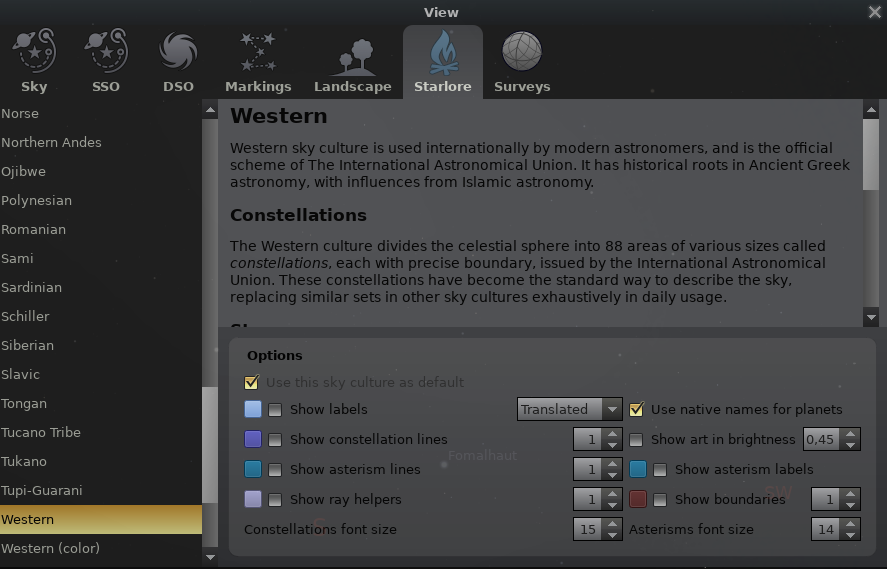
\includegraphics[width=0.75\textwidth]{view_dialog_starlore_tab.png}
\caption{View Settings Window: Starlore Tab}
\label{fig:gui:view:starlore}
\end{figure}

The Starlore tab of the View window (Fig.~\ref{fig:gui:view:starlore})
controls which culture's constellations and bright star names will be
used in the main display.  Some cultures have constellation art (e.g.,
Western and Inuit), and the rest do not. Configurable options include
\begin{description}
\item[Use this sky culture as default] Activate this option to load
  this sky culture when Stellarium starts.
\item[Show labels] Activate display of constellation labels, like
  \guibutton{0.6}{bt_constellation_name.png} or \keys{V}. You can further
  select whether you want to display abbreviated, original or
  translated names.
\item[Show lines with thickness\ldots] Activate display of stick
  figures, like \guibutton{0.6}{bt_constellation.png} or \keys{C}, and you
  can configure constellation line thickness here.
\item[Show asterism lines\ldots] Activate display of asterism stick figures   
  (like the shortcut \keys{Alt+A}), and you can configure asterism line thickness here.\newFeature{0.16.0}
\item[Show ray helpers\ldots] Activate display of special navigational lines which 
  connect stars often from different constellations (like the shortcut \keys{Alt+R}),
  and you can configure thickness of those lines here.\newFeature{0.17.0}
\item[Show boundaries] Activate display of constellation boundaries,
  like \keys{B}. Currently, boundaries have been defined only for
  ``Modern'' sky cultures.
\item[Use native names for planets] If provided, show the planet names
  as used in this sky culture (also shows modern planet name for
  reference). %% TODO THIS FEATURE NEEDS SOME REWORK!
\item[Show art in brightness\ldots] Activate display of constellation
  art (if available), like \guibutton{0.6}{bt_constellation_art.png} or
  \keys{R}. You can also select the brightness here.
\item[Show asterism labels] Activate display of asterism labels, like \keys{Alt+V}.\newFeature{0.16.0}
\end{description}

\subsubsection{Select single constellations}
\label{sec:starlore:singleConstellations}

Some presenters may want to explain a particular storyline about the
constellations of a sky culture, which includes showing single
constellations or showing a sequence of appearing constellations. To
achieve this, first activate the single constellation mode (see
section~\ref{fig:gui:configuration:tools}).  Then, click on a star
which is part of a constellation line set. Click
another star which is part of another constellation to show that one.

If you explain a sky culture where constellations also have borders
defined, a click anywhere in the constellation area is enough.  For
other sky cultures, clicking onto a star which is not member of a
constellation line will display all constellations.

Press \keys{W} to remove all but the last selected constellation.
If you had deleted selection (right mouse click) before pressing \keys{W},
all constellations are hidden.
Press \keys{W} again to also hide the single displayed one, or click
another star to select the next constellation. If you need to keep the
single constellation visible, select the currently selected star again
to select it again.  Press \keys{Alt+W} to show all constellations.

With a little training, you will be able to give inspiring
constellation tours.

\subsection{The Surveys Tab}
\label{sec:gui:view:surveys}

\begin{figure}[htbp]
\centering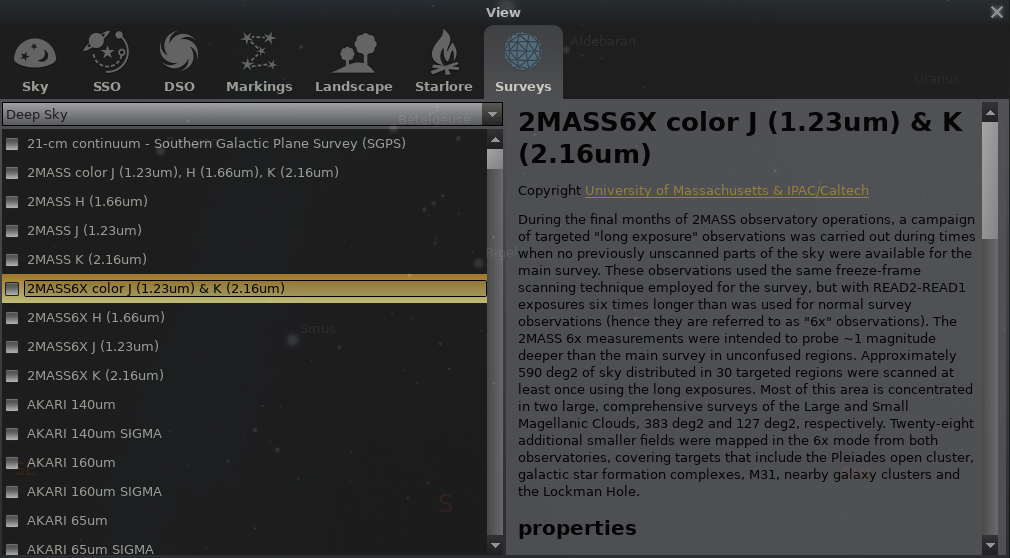
\includegraphics[width=0.75\textwidth]{view_dialog_surveys_tab.png}
\caption{View Settings Window: Surveys Tab}
\label{fig:gui:view:surveys}
\end{figure}

The Surveys tab\newFeature{0.18.0} (Fig.~\ref{fig:gui:view:surveys}) allows to toggle the
visibility of online sky or solar system surveys (see chapter~\ref{ch:surveys}
for description of the surveys format).  Currently, only HiPS surveys are
supported.

On the left side of the window we see the list of available surveys from
the configured sources (See section \ref{sec:config.ini:hips} for how to
change the default sources).  On the right side a description of the selected
survey and its properties are displayed.

Surveys are grouped by types. The top combobox allows to filter the listed
surveys according to a given type (Deep Sky or Solar System).

You can toggle the visibility of a survey by checking the box on the left
of the survey name in the list.  (Note that as of v0.18.0, only a single deep
sky survey can be rendered at a time, so it makes no sense to select more than one in
the list!) Once a survey is visible you should be able to see its loading
status in the loading bar area of the sky view.

Deep sky surveys will be rendered aligned with the sky view, while solar system
surveys automatically map on the proper body.


\section{The Search Window}
\label{sec:gui:search}

\begin{figure}[p]
\centering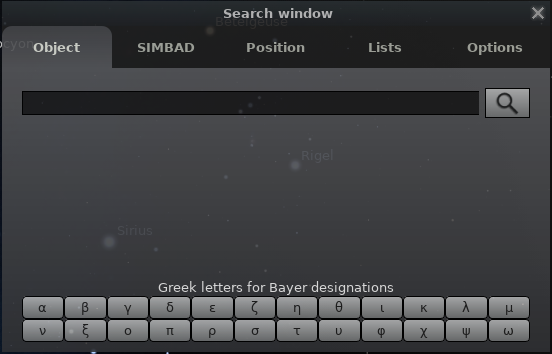
\includegraphics[width=0.68\textwidth]{search_dialog.png}
\caption{The Search Window: Object}
\label{fig:gui:search}
\end{figure}

\begin{figure}[p]
\centering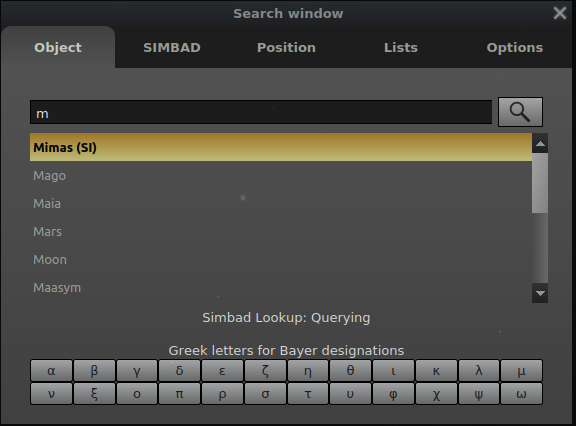
\includegraphics[width=0.68\textwidth]{search_dialog_recent_result.png}
\caption{The Search Window: Object (Recent Searches)}
\label{fig:gui:search:recentSearches}
\end{figure}

\begin{figure}[p]
\centering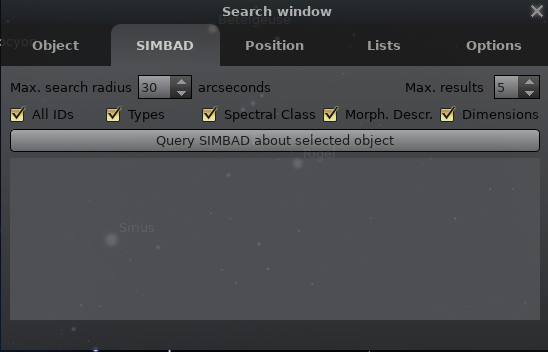
\includegraphics[width=0.68\textwidth,trim=0 30 0 0,clip]{search_dialog_simbad.png}
\caption{The Search Window: SIMBAD}
\label{fig:gui:search:simbad}
\end{figure}

\begin{figure}[p]
\centering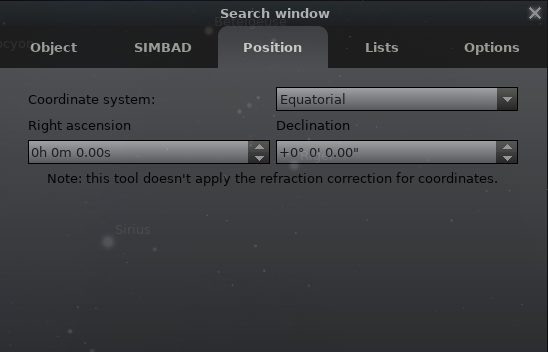
\includegraphics[width=0.68\textwidth,trim=0 40 0 0,clip]{search_dialog_position.png}
\caption{The Search Window: Position}
\label{fig:gui:search:position}
\end{figure}

\begin{figure}[tbp]
\centering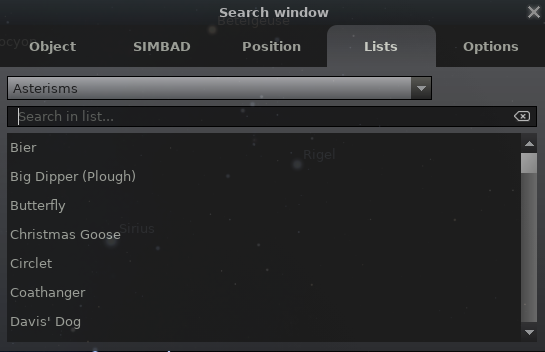
\includegraphics[width=0.68\textwidth]{search_dialog_list.png}
\caption{The Search Window: Lists}
\label{fig:gui:search:lists}
\end{figure}


\begin{figure}[tbp]
\centering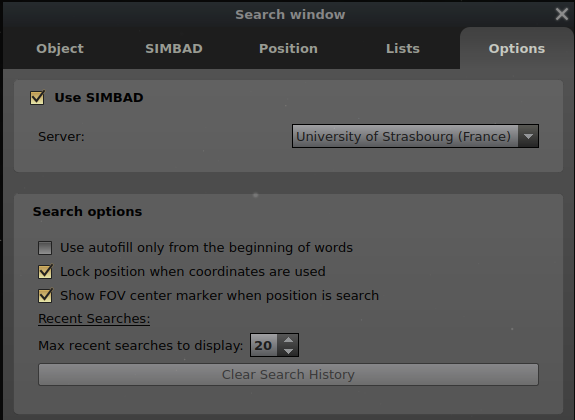
\includegraphics[width=0.68\textwidth]{search_dialog_option.png}
\caption{The Search Window: Options}
\label{fig:gui:search:options}
\end{figure}

\subsection{The Object tab}
\label{sec:gui:SearchWindow:Object}
The Object tab of the Search window provides a convenient way to locate objects
in the sky. Simply type in the name of an object to find, and press
\key{\return}. Stellarium will point you at that object in the sky.

As you type, Stellarium will make a list of objects which contains 
what you have typed so far. The first of the list of matching objects
will be highlighted. If you press the \key{\tab} or \key{\arrowkeydown} key,
the selection will change to the next item in the list.
Pressing the \key{\arrowkeyup} key will bring you to the previous item.
Hitting the \key{\return} key will center on the
currently highlighted object and close the Search window.

For example, suppose we want to locate Saturn's moon Mimas (SI).
Open the Search window (\guibutton[0.5]{2.5}{btd_find.png}, \key{F3}, or \key{Ctrl+F}).
Type the first letter of the name, \emph{m}, to see a list
of objects whose name contains \emph{m}:
\begin{center}
\begin{tabular}{l}
        \emph{M}iranda (UV)\\
        Psa\emph{m}athe (NX)\\
        U\emph{m}briel (UII)\\
        \ldots\\
\end{tabular}
\end{center}

\noindent You may want at this point to have Stellarium rather propose object
names which start with the string you enter. Do that in the Options tab
of this panel (see section~\ref{sec:gui:SearchWindow:Options}).
The search result should update automatically\newFeature{0.20.3}
when you nagivate back to the Object tab.
Now the list is shorter and contains only objects which start
with \emph{m}:
\begin{center}
\begin{tabular}{l}
        \emph{M}ago\\
        \emph{M}aia\\
        \emph{M}ars\\
        \ldots\\
\end{tabular}
\end{center}

\noindent The first item in this list, Mago, is
highlighted. Pressing \key{\return} now would go to Mago, but we want
Mimas (SI). We can either press \key{\tab} or \key{\arrowkeydown} a few times to highlight Mimas (SI)
and then hit \key{\return}, or we can continue to type the name until
it is the first/only object in the list.

After you searched for an object, the next time the Search window opens,\newFeature{0.20.3}
your most recently searched object(s)
will automatically appear in the search result of the Object tab.
For instance, continuing with our example, re-open the Search window's Object tab.
Mimas (SI) should already be populated and highlighted:
\begin{center}
\begin{tabular}{l}
        \textbf{\emph{M}imas (SI)}\\
\end{tabular}
\end{center}

\noindent The Object tab's search result will now prioritize your most recent searches
(which will be shown in \textbf{bold}).\newFeature{0.20.3}
To modify the search results, see section~\ref{sec:gui:SearchWindow:Options}.
From our earlier example, re-enter \emph{m} into the Object tab.
Doing so will generate a slightly different list than before.
In this case, Mimas (SI) will appear first, as shown in Figure~\ref{fig:gui:search:recentSearches}:
\begin{center}
\begin{tabular}{l}
        \textbf{\emph{M}imas (SI)}\\
        \emph{M}ago\\
        \emph{M}aia\\
        \emph{M}ars\\
        \ldots\\
\end{tabular}
\end{center}

\subsection{The SIMBAD tab}
\label{sec:gui:SearchWindow:SIMBAD}
The SIMBAD tab (Fig.~\ref{fig:gui:search:simbad}) provides a
convenient way to fetch and show a set of information for selected
object from the astronomical online database
SIMBAD~\citep{2000A&AS..143....9W}.  If some object is only visible in
a survey or DSS background (see section~\ref{ch:surveys}) and not in
Stellarium's catalogs, you can also set a custom marker (see
section~\ref{sec:tour:markers}), select it and query SIMBAD ``tell me
what's known about objects at this location''.

\subsection{The Position tab}
\label{sec:gui:SearchWindow:Position}
The Position tab (Fig.~\ref{fig:gui:search:position}) provides a convenient way to enter a set
of coordinates.

\subsection{The Lists tab}
\label{sec:gui:SearchWindow:Lists}
The Lists tab (Fig.~\ref{fig:gui:search:lists}) allows selection of an object from predefined
sets.  The number of choices is governed by the loaded DSO catalogs and plug-ins. 
Scroll down the first window to select the type. Click on the name
and Stellarium will center on that object.

\subsection{The Options tab}
\label{sec:gui:SearchWindow:Options}
The Options tab (Fig.~\ref{fig:gui:search:options}) provides a few settings to fine-tune your search experience.

\begin{description}
\item[Use SIMBAD]
When the name of an object to find is typed in the Object
tab and you are connected to the internet and ``Use SIMBAD'' is
ticked, Stellarium will search the SIMBAD on-line databases for its
coordinates. You can then click the \guibutton{0.6}{bt_search.png} button or press \key{\return}.
Stellarium will point you at that object in the sky even if there is no
object displayed on the screen. The SIMBAD server being used can be
selected from the scroll window.
\begin{description}
\item[Server:] for server selection
\end{description}
\end{description}

\begin{description}
\item[Search Options] group allows for changes in the search result behaviour.
\begin{description}
\item[Use autofill only from the beginning of words] when checked, will 
search for object names that begins with the same letters as your input. 
Example provided in section~\ref{sec:gui:SearchWindow:Object}. 
\item[Lock position when coordinates are used]
\item[Show FOV center marker when position is search]
\end{description}        
\end{description}

\begin{description}
\item[Recent Searches]group allows modification to your recent search data\newFeature{0.20.3}. 
Any changes here will automatically update the search results displayed in the Object tab. 
Example provided in section~\ref{sec:gui:SearchWindow:Object}.
\begin{description}
\item[Max items to display] amount of \emph{recent searches} that can appear in the search result
\item[\guibutton{1.0}{uibtDelete.png}] button deletes your recent search history
\end{description}
\end{description}

\section{The Astronomical Calculations Window}
\label{sec:gui:AstroCalc}

This window \newFeature{0.15.0} provides advanced functionality, some of which is still under development.
You can call it by pressing \key{F10} or the button \guibutton{0.6}{btd_astrocalc.png} on the left menu bar. 
The Astronomical Calculations window shows eight tabs with different functionality.

Most tabs allow \newFeature{0.18.3} exporting computed data to XLSX (Excel) files in addition to CSV files, and
graphs can be exported \newFeature{0.22.2} as PNG files.

\subsection{The Positions Tab}
\label{sec:gui:AstroCalc:Positions}

This tab \newFeature{0.16.0} shows equatorial J2000.0 or horizontal positions, magnitudes and additional parameters 
(e.g.\ surface brightness for deep-sky objects or angular separation for double stars) for various 
lists of celestial objects above the horizon at the simulated time, filtered by magnitude. 
Double-clicking on an entry brings the object into focus (Fig.~\ref{fig:gui:AstroCalc:Positions}). 
You may also export the list of positions into an XLSX or CSV file.

\begin{figure}[htbp]
	\centering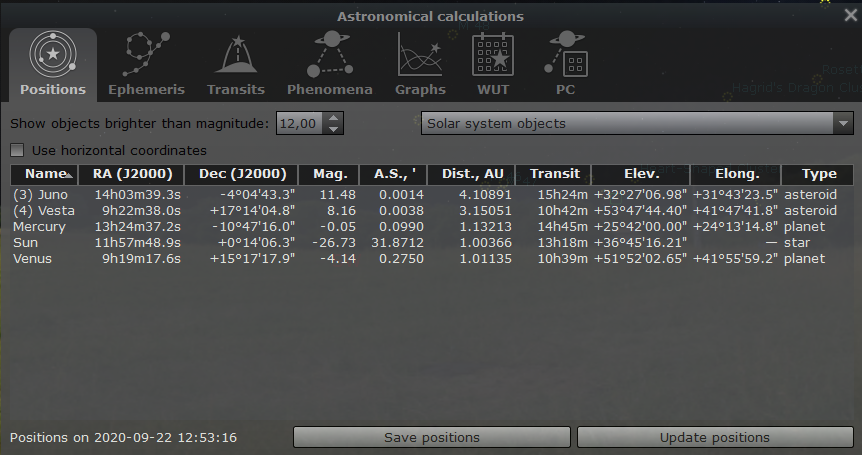
\includegraphics[width=0.8\textwidth]{astrocalc_dialog_positions_tab.png}
	\caption{Astronomical Calculations (AstroCalc): Celestial positions / Seen now}
	\label{fig:gui:AstroCalc:Positions}
\end{figure}

This tab \newFeature{0.22.0} is split into 2 subtabs: ``Seen now'' and ``Major planets''.
The ``Major planets'' subtab (Fig.~\ref{fig:gui:AstroCalc:Positions:MajorPlanets}) shows a table
with heliocentric ecliptic positions of the major planets and a graphical representation of these positions
(in polar coordinates). You may also export the list of positions into an XLSX or CSV file.

\begin{figure}[htbp]
	\centering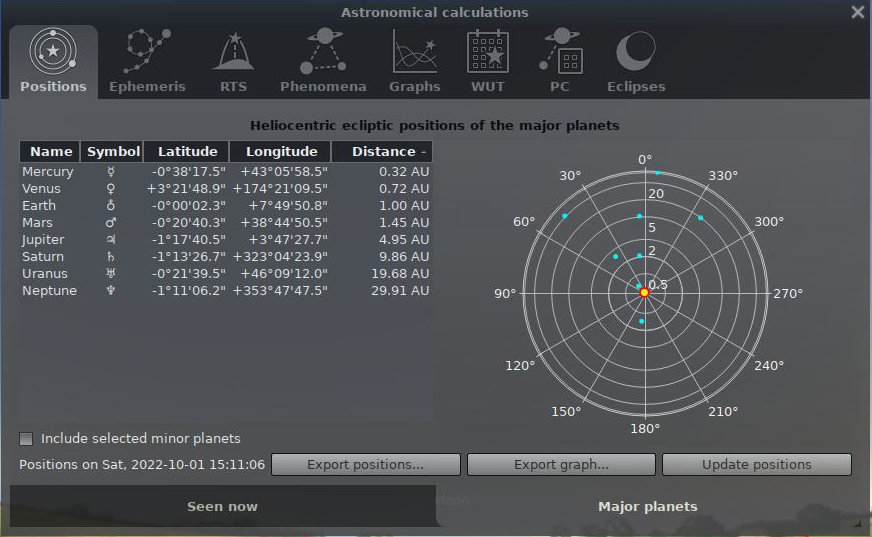
\includegraphics[width=0.8\textwidth]{astrocalc_dialog_positions_mp_tab.png}
	\caption{Astronomical Calculations (AstroCalc): Celestial positions / Major Planets}
	\label{fig:gui:AstroCalc:Positions:MajorPlanets}
\end{figure}

\subsection{The Ephemeris Tab}
\label{sec:gui:AstroCalc:Ephemeris}

Select an object, start and end time, and compute an ephemeris (list of positions and magnitudes evolving over time) for that object. 
The positions are marked in the sky with yellow disks (Fig.~\ref{fig:gui:AstroCalc:Ephemeris}). 

\begin{figure}[p]
	\centering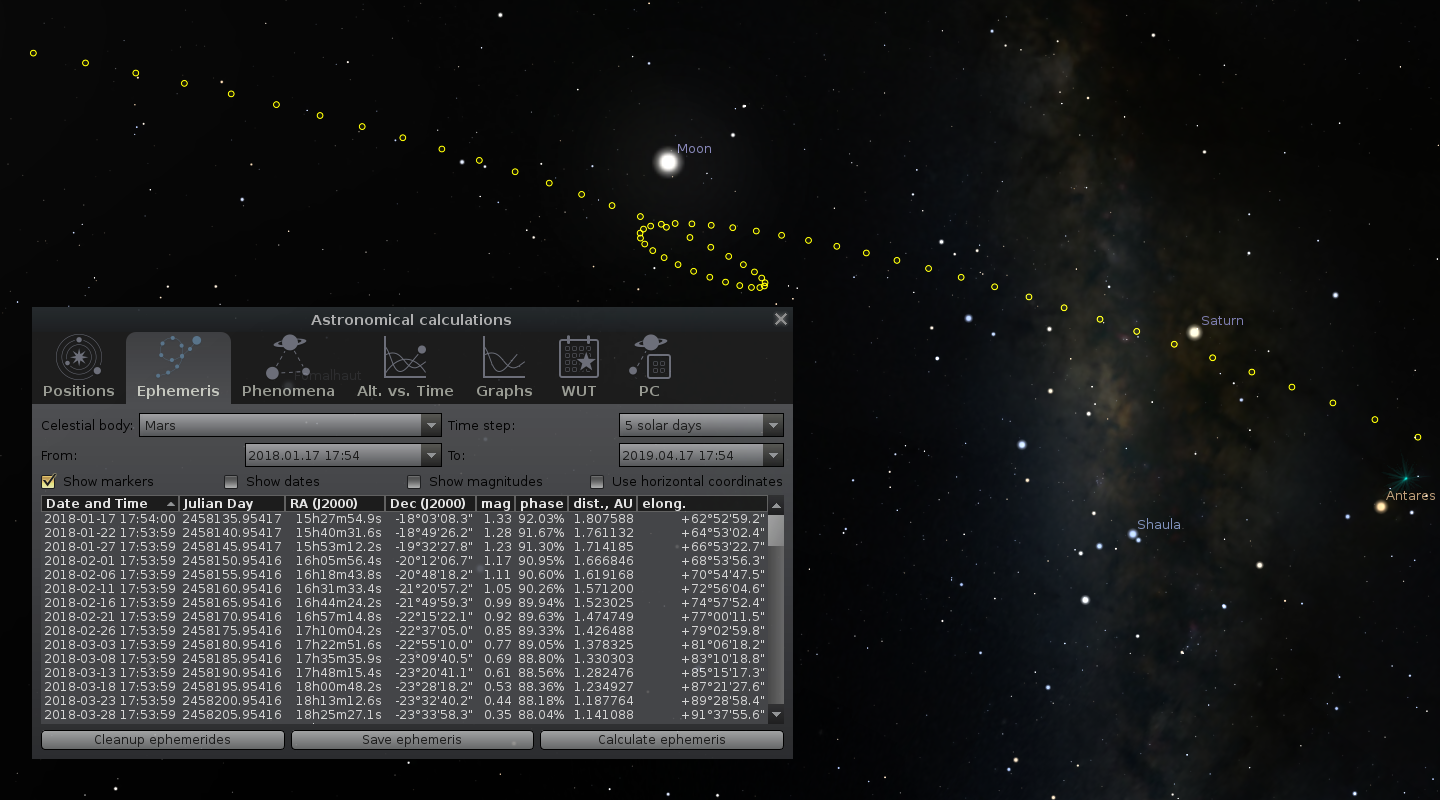
\includegraphics[width=0.8\textwidth,trim=0 15 0 15,clip]{astrocalc_dialog_ephemeris_tab.png}
	\caption{Astronomical Calculations (AstroCalc): Plot trace of planet}
	\label{fig:gui:AstroCalc:Ephemeris}
\end{figure}

\begin{figure}[p]
	\centering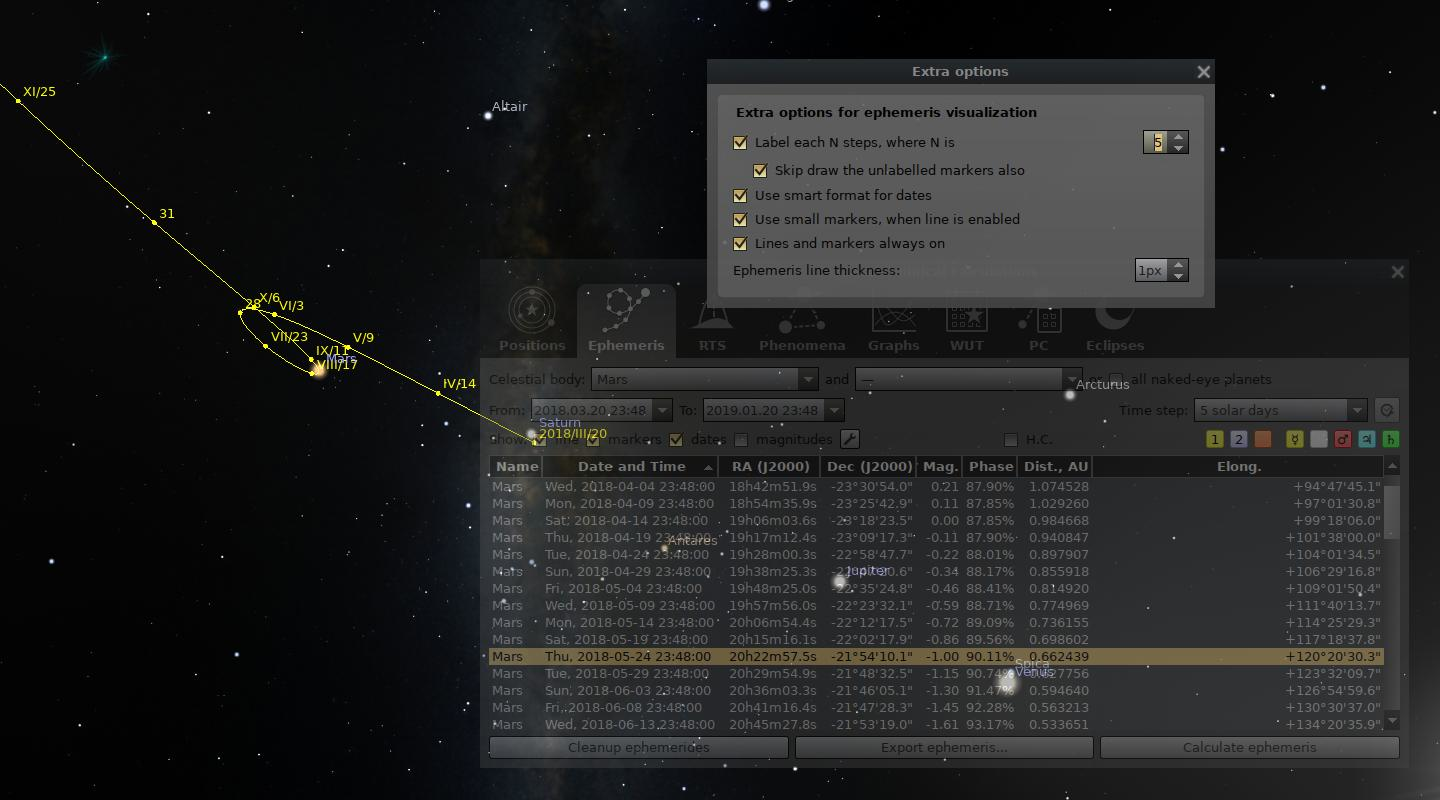
\includegraphics[width=0.8\textwidth,trim=0 15 0 15,clip]{astrocalc_dialog_ephemeris_extra.png}
	\caption{Astronomical Calculations (AstroCalc): Extra options for ephemeris}
	\label{fig:gui:AstroCalc:Ephemeris:Extra}
\end{figure}

\begin{figure}[p]
	\centering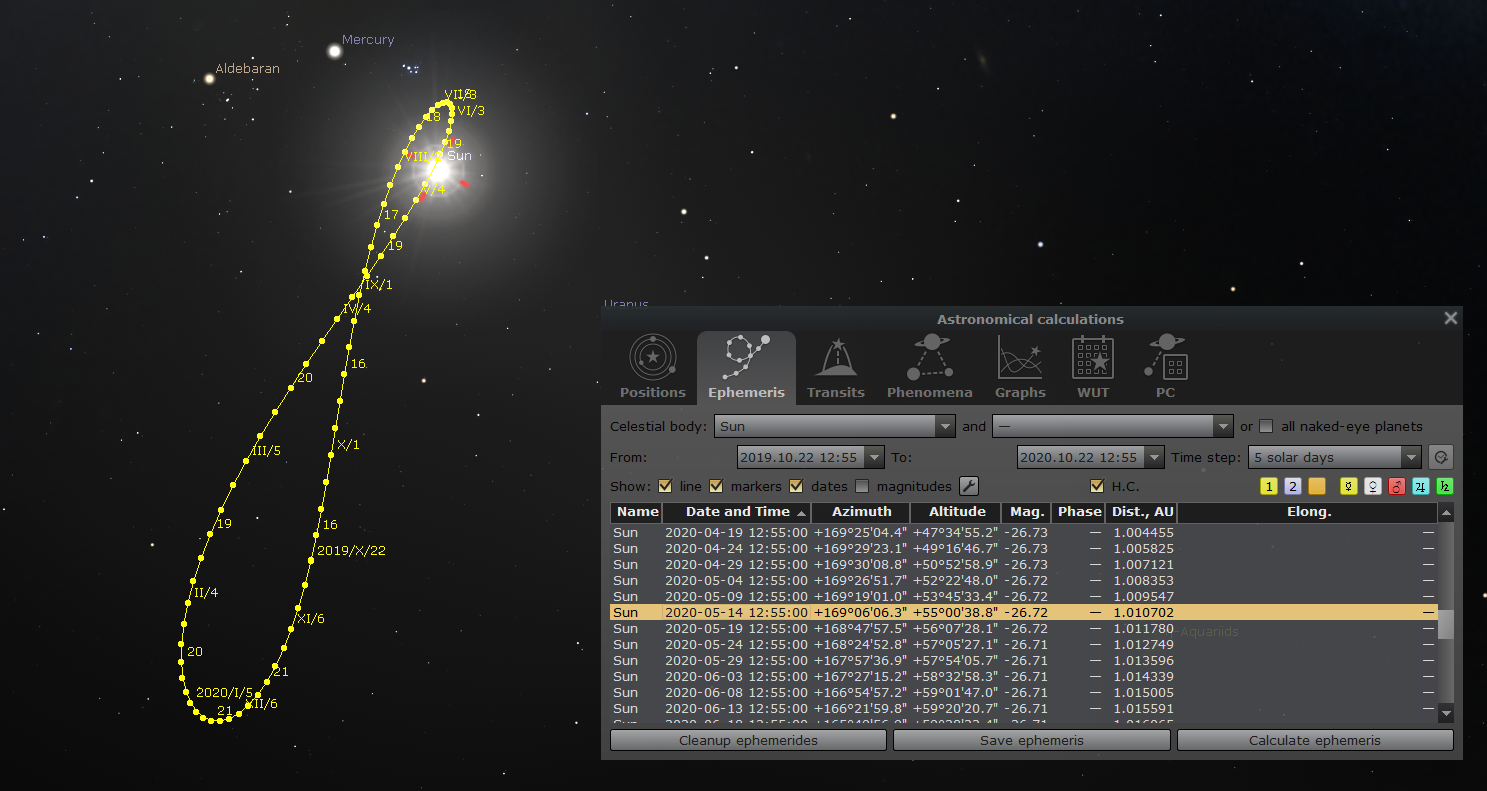
\includegraphics[width=0.8\textwidth,trim=0 15 0 15,clip]{astrocalc_dialog_ephemeris_analemma.png}
	\caption{Astronomical Calculations (AstroCalc): Analemma on the Earth}
	\label{fig:gui:AstroCalc:Ephemeris:Analemma}
\end{figure}


When you click on a date, an orange disk indicates this date and/or magnitude. 
Double-clicking sets the respective date and brings the object to focus. 
Dates and/or magnitudes will show up near position markers when \emph{Show dates} 
and/or \emph{Show magnitudes} checkboxes are active. \newFeature{0.19.2} 
To show a line between markers please tick checkbox \emph{Show line}. 
You may customize the format of displayed data near markers and their frequency in the \emph{Extra options} window (Fig.~\ref{fig:gui:AstroCalc:Ephemeris:Extra}).
You can also\newFeature{0.19.2} define the color of markers and enable display markers for all naked-eye visible planets.

You can export the calculated ephemeris into an XLSX or CSV file. 

\begin{figure}[p]
	\centering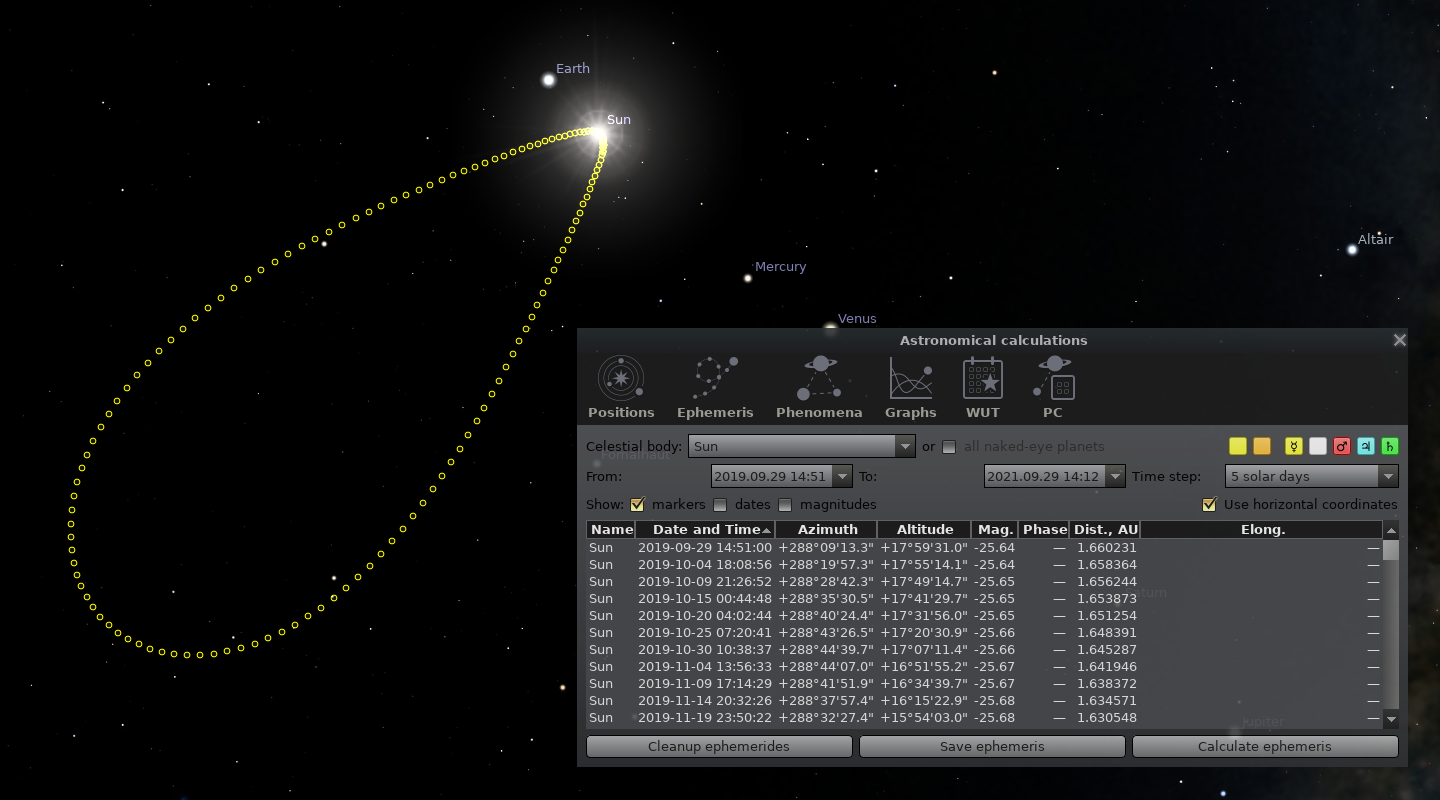
\includegraphics[width=0.8\textwidth]{astrocalc_dialog_ephemeris_analemma_mars.png}
	\caption{Astronomical Calculations (AstroCalc): Analemma on Mars}
	\label{fig:gui:AstroCalc:Ephemeris:AnalemmaMars}
\end{figure}

\begin{figure}[p]
	\centering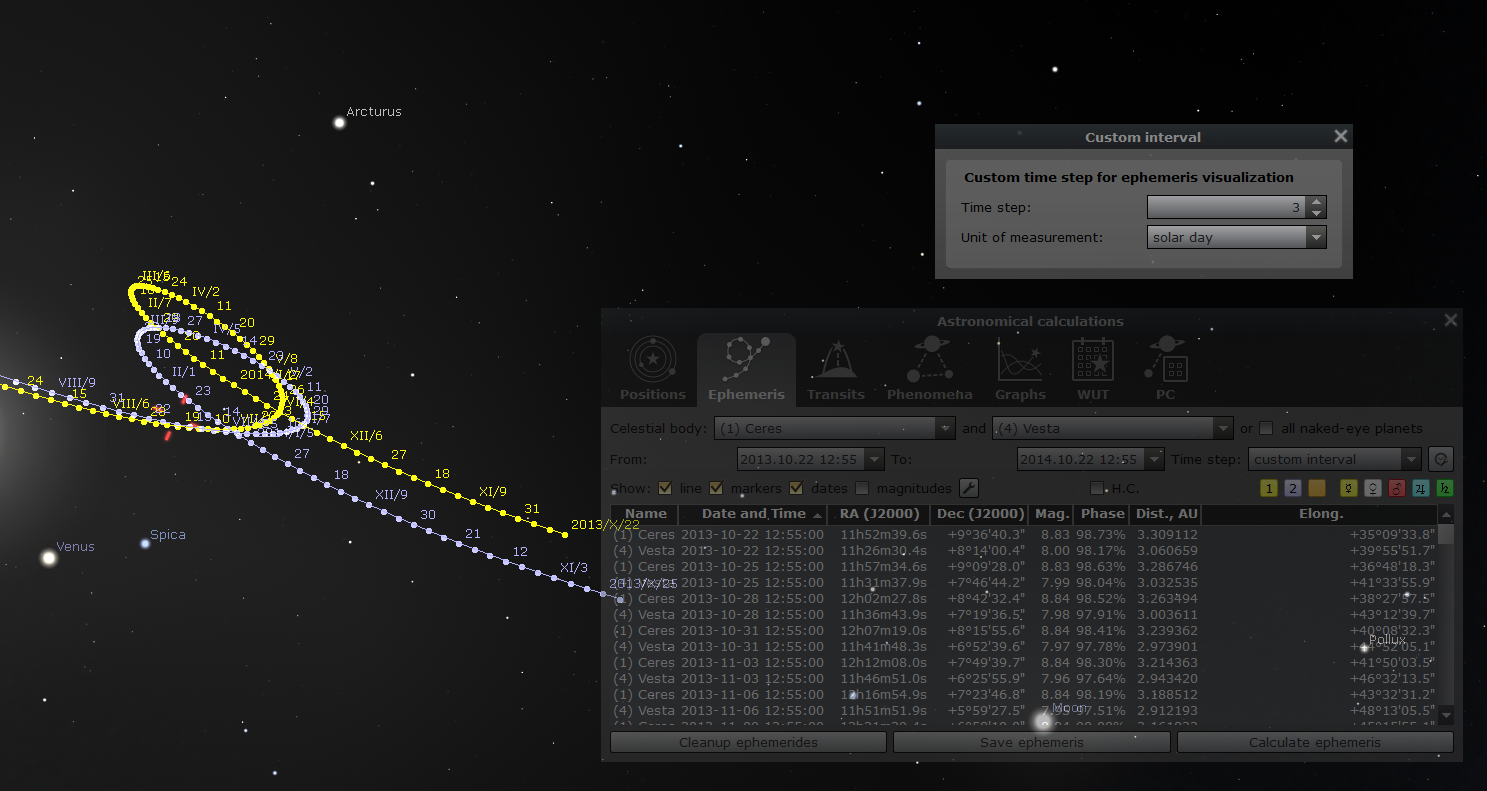
\includegraphics[width=0.8\textwidth]{astrocalc_dialog_ephemeris_asteroids.png}
	\caption{Astronomical Calculations (AstroCalc): Two asteroids nearby to one place}
	\label{fig:gui:AstroCalc:Ephemeris:Asteroids}
\end{figure}

Another interesting option in this tool: using horizontal coordinates for plotting traces of the Solar system objects. 
In this mode, the circle marks are not linked to the sky, but to the horizontal coordinate system.
For example, you can get an analemma of the Sun for any location (Fig.~\ref{fig:gui:AstroCalc:Ephemeris:Analemma}
and \ref{fig:gui:AstroCalc:Ephemeris:AnalemmaMars}), 
or observe the visibility of Mercury, Venus or a comet in the twilight sky.

You can \newFeature{0.20.3}  draw an ephemeris of 
two objects at the same time and define custom time step for the ephemeris 
(Fig.~\ref{fig:gui:AstroCalc:Ephemeris:Asteroids}).

\subsection{The ``Risings, Transits, and Settings'' (RTS) Tab}
\label{sec:gui:AstroCalc:RTS}

\begin{figure}[htbp]
	\centering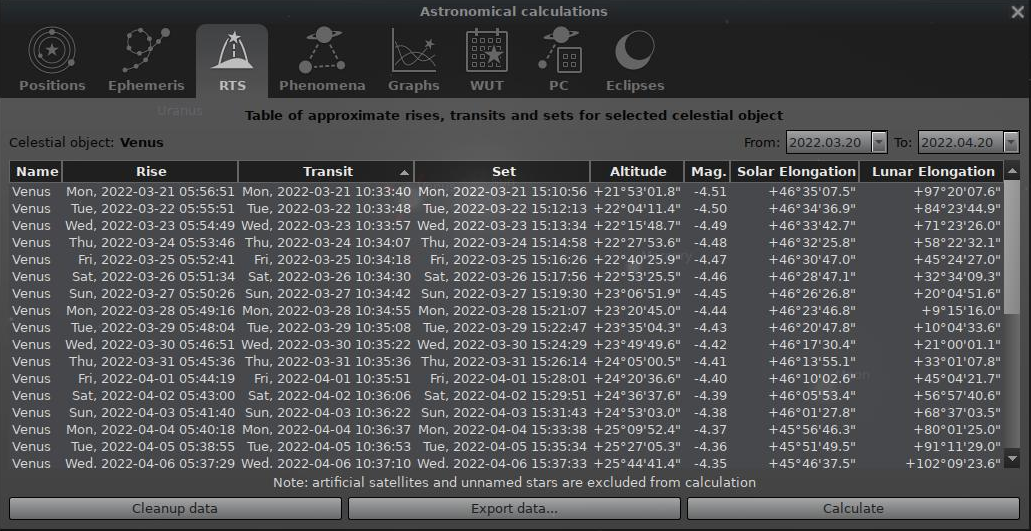
\includegraphics[width=0.8\textwidth]{astrocalc_dialog_transits_tab.png}
	\caption{Astronomical Calculations (AstroCalc): Risings, transits, and settings of selected celestial object}
	\label{fig:gui:AstroCalc:RTS}
\end{figure}

\noindent This \newFeature{0.19.3} tab allows you to compute meridian transits and
\newFeature{0.22.0} rising and setting times of selected celestial object 
(except unnamed stars and artificial satellites) for a specific date range. 
The tool is useful for planning observations, and it suggests the best time and conditions 
for visual observations or astrophotography (Fig.~\ref{fig:gui:AstroCalc:RTS}). 

You may also export the list of transits into an XLSX or CSV file.

\subsection{The Phenomena Tab}
\label{sec:gui:AstroCalc:Phenomena}

This tab allows you to compute phenomena like conjunctions, oppositions, 
occultations and eclipses (in special cases) between planetary objects 
(Fig.~\ref{fig:gui:AstroCalc:Phenomena}). 
In addition, \newFeature{0.19.3} it provides computation of greatest 
elongations for the inner planets and stationary points for all planets, and,
for all Solar system bodies except the moons, we also compute perihelia and aphelia.

You can export the calculated phenomena into an XLSX or CSV file.

\begin{figure}[tbp]
\centering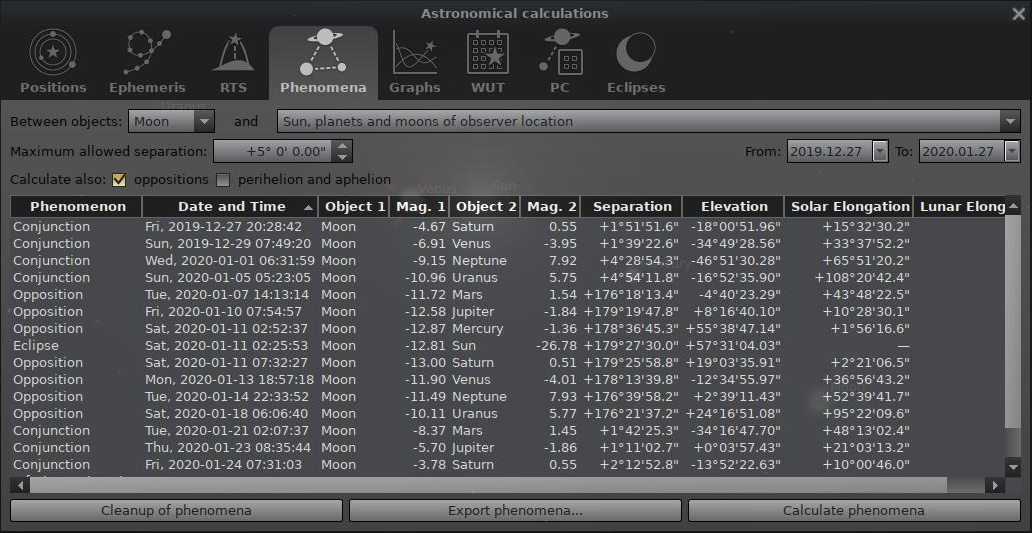
\includegraphics[width=0.8\textwidth]{astrocalc_dialog_phenomena_tab.png}
\caption{Astronomical Calculations (AstroCalc): Phenomena}
\label{fig:gui:AstroCalc:Phenomena}
\end{figure}

Four columns in the table may be helpful for planning observation of phenomena:
\begin{description}
  \item[solar elongation] angular distance from the Sun\newFeature{0.18.2/.3}
  \item[lunar elongation] angular distance from the Moon\newFeature{0.18.2/.3}
  \item[mag. 1] magnitude of first object\newFeature{0.19.3}
  \item[mag. 2] magnitude of second object\newFeature{0.19.3}
\end{description}


\subsection{The Graphs Tab}
\label{sec:gui:AstroCalc:Graphs}

\begin{figure}[p]
\centering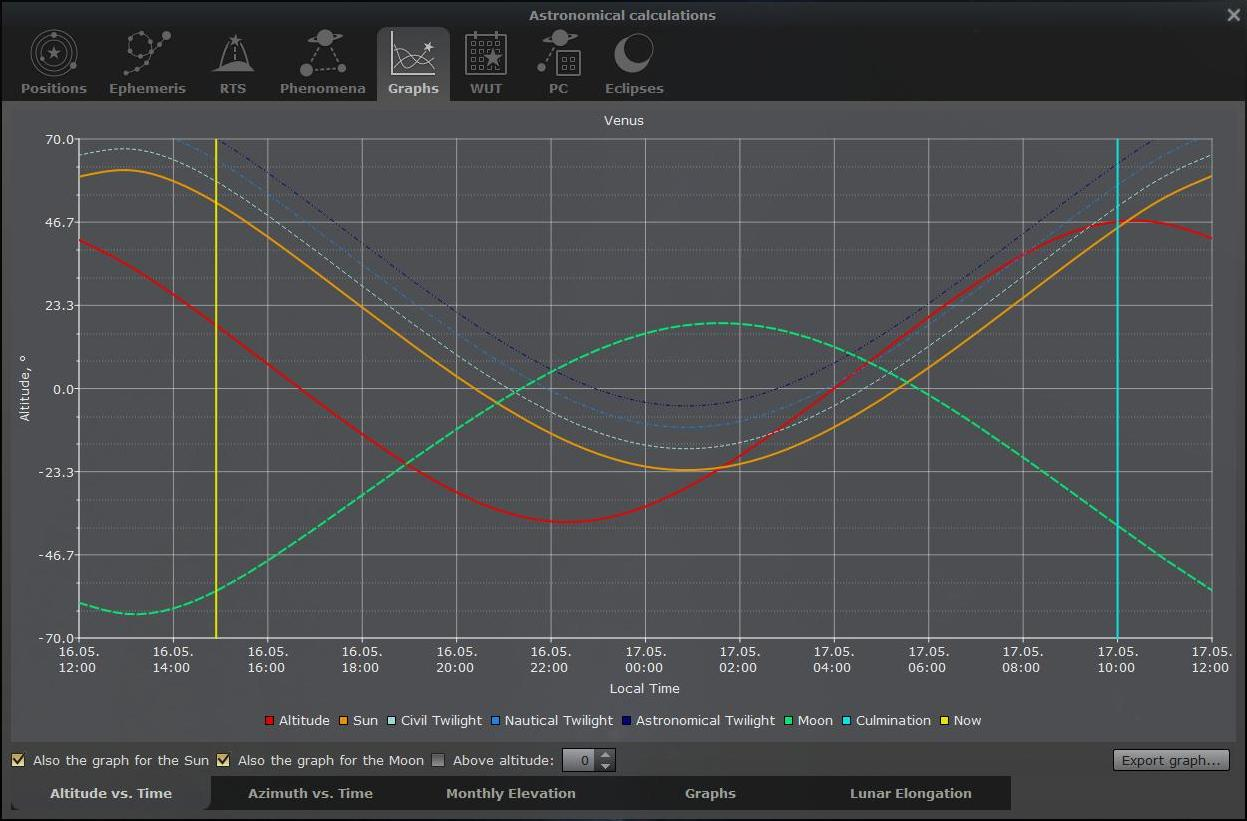
\includegraphics[width=0.7\textwidth]{astrocalc_dialog_graphs_tab_altvstime.jpg}
\caption{Astronomical Calculations (AstroCalc): Graphs / Altitude vs.\ Time}
\label{fig:gui:AstroCalc:Graphs:AltVsTime}
\end{figure}
\begin{figure}[p]
\centering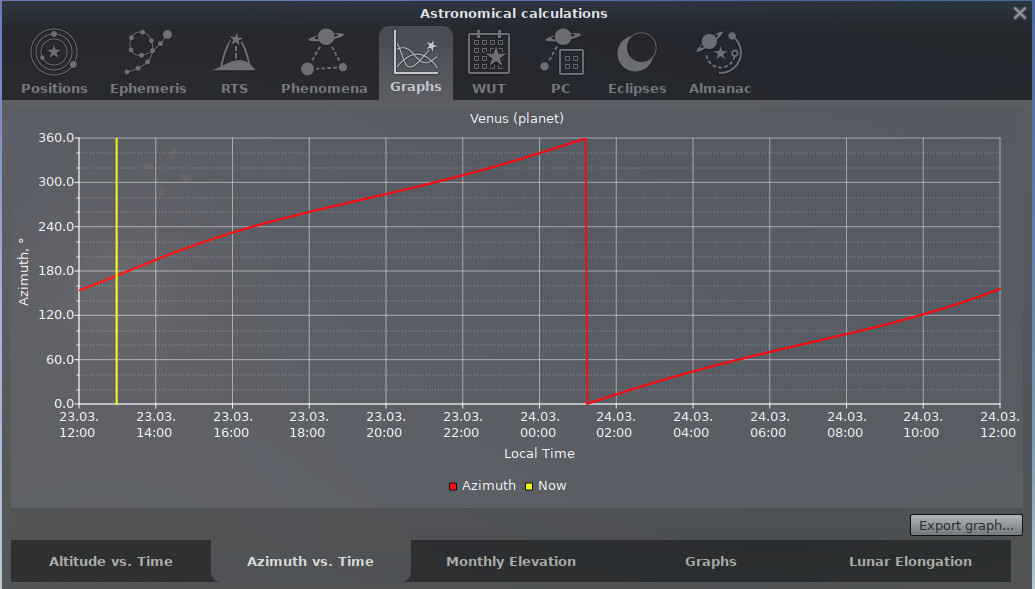
\includegraphics[width=0.7\textwidth]{astrocalc_dialog_graphs_tab_azivstime.jpg}
\caption{Astronomical Calculations (AstroCalc): Graphs / Azimuth vs.\ Time}
\label{fig:gui:AstroCalc:Graphs:AziVsTime}
\end{figure}

\begin{figure}[p]
\centering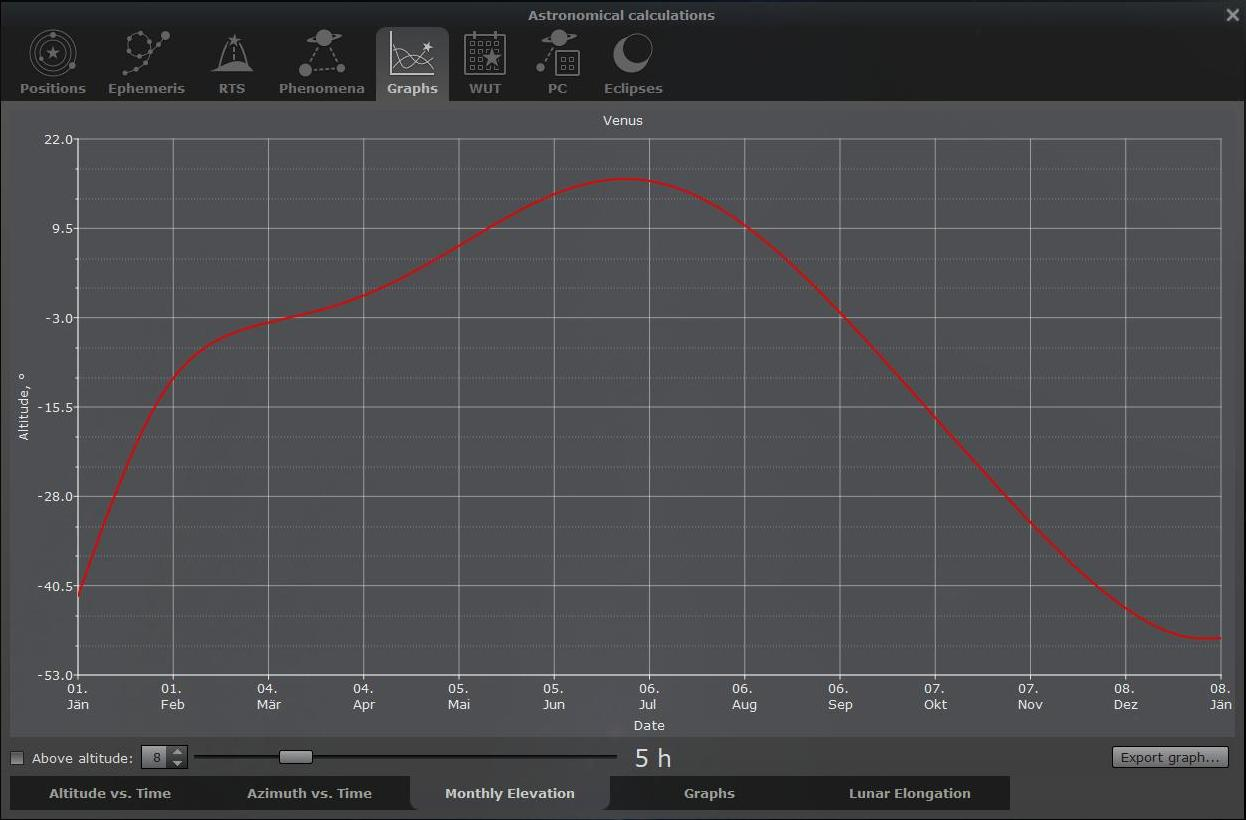
\includegraphics[width=0.65\textwidth]{astrocalc_dialog_graphs_tab_me.jpg}
\caption{Astronomical Calculations (AstroCalc): Graphs / Monthly Elevation}
\label{fig:gui:AstroCalc:Graphs:ME}
\end{figure}


This tab\newFeature{0.18.3} provides on several sub-tabs
\newFeature{0.19.0} graphs which are helpful for monthly observation
planning of deep-sky objects and analysis of changes between objects
or changes of their positions. Clicking \newFeature{0.22.2} in the
graph sets the time at that point, and setting the mouse onto a graph
displays values at this point. However, most graphs are intended for a
rapid overview and are plotted using an interpolating spline through sparse samples,
so do not expect highest accuracy. 

\subsubsection{The ``Altitude vs.\ Time'' Subtab}
\label{sec:gui:AstroCalc:Graphs:AltVsTime}
  
On this subtab (the first subtab and default view in the Graphs tab) you can compute the geometrical altitude of the currently selected object 
on the currently set date and draw it as a graph (Fig.~\ref{fig:gui:AstroCalc:Graphs:AltVsTime}).

Optional graphs for the Sun (with lines for civil, nautical and astronomical twilight) and the Moon (dashed) are also available.

\subsubsection{The ``Azimuth vs.\ Time'' Subtab}
\label{sec:gui:AstroCalc:Graphs:AziVsTime}
  
On this subtab \newFeature{0.19.1} you can compute the geometrical azimuth of the currently selected object 
on the currently set date and draw it as a graph (Fig.~\ref{fig:gui:AstroCalc:Graphs:AziVsTime}).
    
\subsubsection{The ``Monthly Elevation'' Subtab}
\label{sec:gui:AstroCalc:Graphs:ME}

This subtab \newFeature{0.18.0} can show a ``Monthly Elevation'' graph for the current year at the selected time.
This tool was introduced for planning yearly observations (Fig.~\ref{fig:gui:AstroCalc:Graphs:ME}).

\subsubsection{The ``Graphs'' Subtab}
\label{sec:gui:AstroCalc:Graphs:Graphs}
    
\begin{figure}[p]
\centering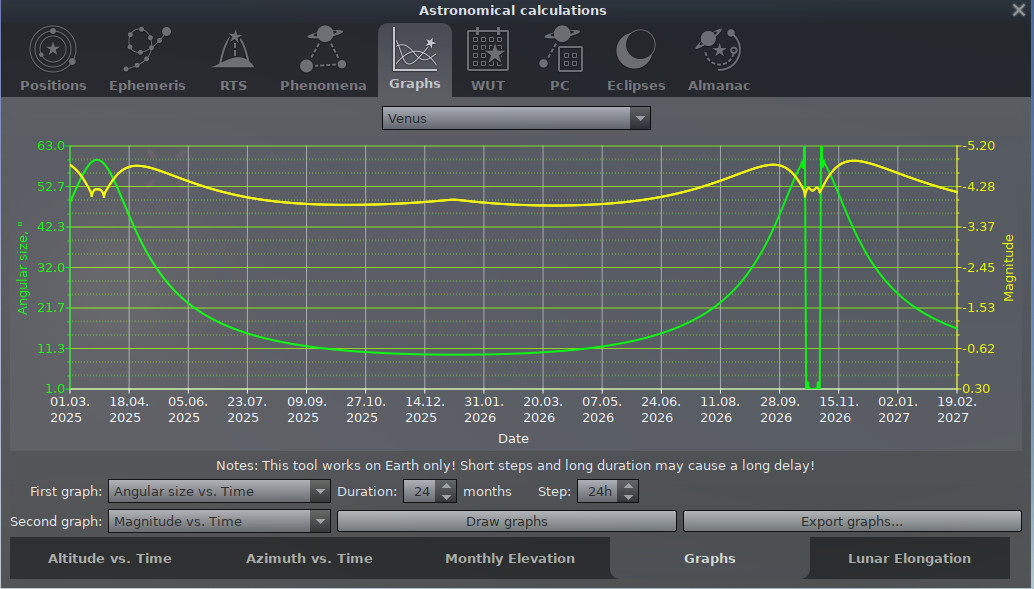
\includegraphics[width=0.65\textwidth]{astrocalc_dialog_graphs_tab_graphs.jpg}
\caption{Astronomical Calculations (AstroCalc): Graphs}
\label{fig:gui:AstroCalc:Graphs:Graphs}
\end{figure}
  
This subtab \newFeature{0.16.0} can show two functions over time for
the current month or for up to 30 years\newFeature{0.19.3/0.22.2} and draw graphs
for them in one screen (Fig.~\ref{fig:gui:AstroCalc:Graphs:Graphs}).
You can select from
\begin{itemize}
\item Magnitude vs. Time
\item Phase vs. Time
\item Distance vs. Time 
\item Elongation vs. Time 
\item Angular size vs. Time
\item Phase angle vs. Time
\item Heliocentric distance vs. Time\newFeature{0.18.2}
\item Transit altitude vs. Time\newFeature{0.19.0}
\item Right ascension vs. Time\newFeature{0.19.3}
\item Declination vs. Time\newFeature{0.19.3}
\end{itemize}

This tool may be very helpful for educational and statistics purposes.%
	\footnote{The idea for this tool has been obtained from \program{SkytechX}: \url{http://www.skytechx.eu/}}
For example, the magnitude curve for Jupiter's moons shows occasional dips where the moon is in Jupiter's shadow.
However, while for most graphs a sampling interval of 24 hours should be sufficient (i.e., 1 value per day),
for this graph you may want to reduce the sampling interval \newFeature{0.22.2} to 1 or 2 hours to avoid missing those eclipses by \indexterm{undersampling}.
Of course, such high density takes much longer to compute, so you should avoid plotting this curve for many years,
or expect a long delay where the program may seem unresponsive.
	
\subsubsection{The ``Lunar Elongation'' Subtab}
\label{sec:gui:AstroCalc:Graphs:LE}

\begin{figure}[p]
\centering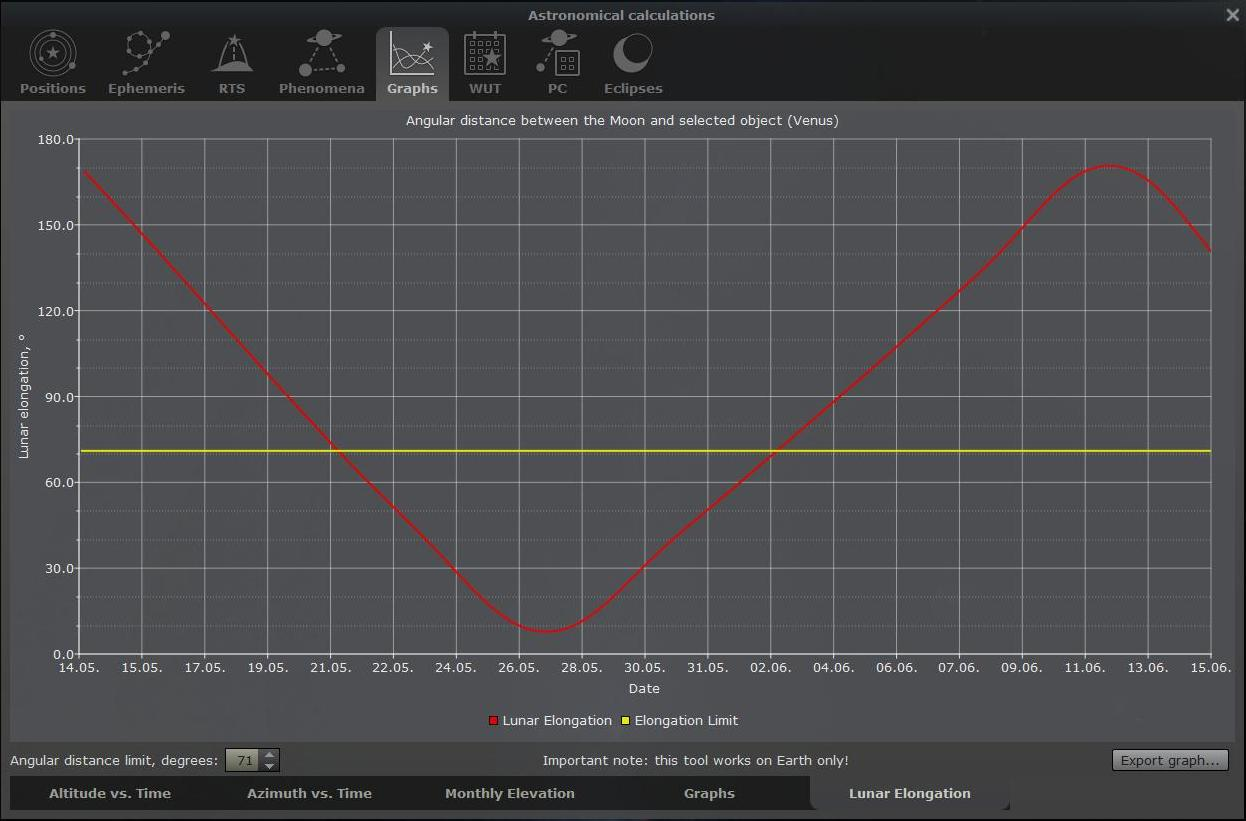
\includegraphics[width=0.65\textwidth]{astrocalc_dialog_graphs_tab_ad.jpg}
\caption{Astronomical Calculations (AstroCalc): Graphs / Lunar Elongation}
\label{fig:gui:AstroCalc:Graphs:LE}
\end{figure}

This subtab (Fig.~\ref{fig:gui:AstroCalc:Graphs:LE})
\newFeature{0.18.3} can show a ``Lunar Elongation''
graph --- the angular distance between the Moon
and the selected object (for example some deep-sky object) for the
nearest 30 days. This tool was introduced for planning monthly
observations.

\subsection{The ``What's Up Tonight'' (WUT) Tab}
\label{sec:gui:AstroCalc:WUT}

The ``What's Up Tonight'' (WUT) tool\newFeature{0.16.0}%
	\footnote{This tool has been partially ported from the \program{KStars} planetarium: \url{https://edu.kde.org/kstars/}}
 displays a list of objects that will be visible at night for the current date and location.

\begin{figure}[p]
\centering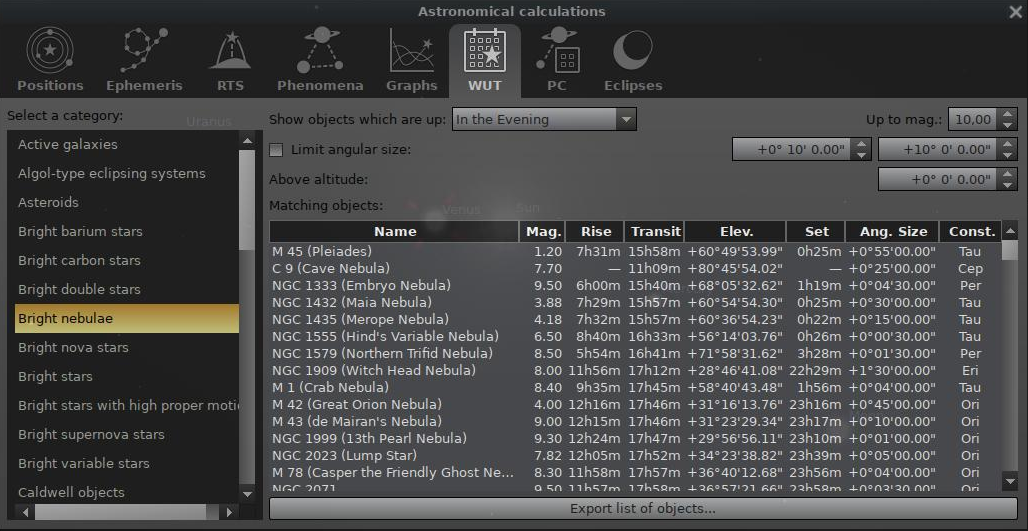
\includegraphics[width=0.8\textwidth]{astrocalc_dialog_wut_tab.png}
\caption{Astronomical Calculations (AstroCalc): What's Up Tonight (WUT)}
\label{fig:gui:AstroCalc:WUT}
\end{figure}

\begin{figure}[p]
\centering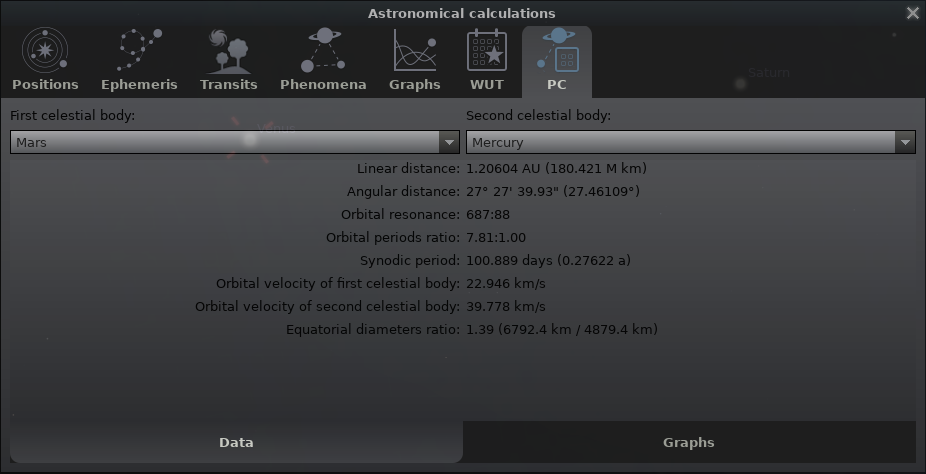
\includegraphics[width=0.8\textwidth]{astrocalc_dialog_pc_tab.png}
\caption{Astronomical Calculations (AstroCalc): Planetary Calculator (PC), Data Tab}
\label{fig:gui:AstroCalc:PC:Data}
\end{figure}
\begin{figure}[p]
\centering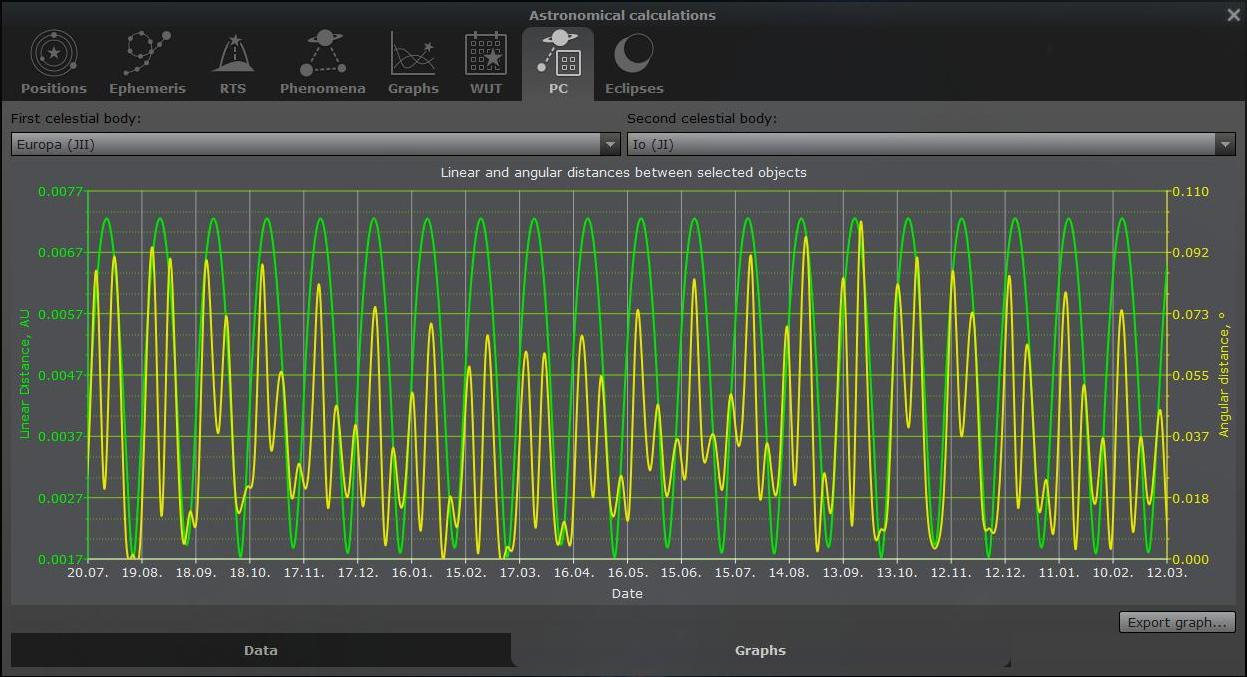
\includegraphics[width=0.8\textwidth]{astrocalc_dialog_pc_graphs_tab.jpg}
\caption{Astronomical Calculations (AstroCalc): Planetary Calculator (PC), Graphs Tab}
\label{fig:gui:AstroCalc:PC:Graphs}
\end{figure}

The objects are organized into type categories. Select an object type in the box labeled 
\emph{Select a Category}, and all objects of that type which are above the horizon on the selected night 
will be displayed in the box labeled \emph{Matching Objects}. For example, in the screenshot, 
the Planets category has been selected, and three planets which are up in the selected night are displayed (Jupiter, Mars and Mercury). 

By default, the WUT will display objects which are above the horizon between sunset and midnight (i.e.\ \emph{in the evening}). 
You can choose to show objects which are up between midnight and dawn (\emph{in the morning}), 
\emph{around midnight}, 
or any time between dusk and dawn (\emph{any time tonight}) using the combobox near the top of the window. 
You can also choose to see only those objects that are brighter than a certain magnitude by 
setting a minimum magnitude using the \emph{Show objects brighter than magnitude} spinbox. 
You may center an object from the right list in the sky map just by selecting it.

Note that only DSO from catalogs which you have selected in the DSO panel (section~\ref{sec:gui:view:dso}) will be found.

In version 0.18.3 \newFeature{0.18.3} this tool has been refactored: the tool for searching items from list of \emph{Matching Objects} was removed,
the filter for magnitudes was moved to the right, and we added a new filter here to limit the range of acceptable angular sizes of matched objects.
In addition to the names we added 5 new sortable columns: magnitude, rising time, transit time, setting time and angular size of object.



\subsection{The ``Planetary Calculator'' (PC) Tab}
\label{sec:gui:AstroCalc:PC}

The ``Planetary Calculator'' (PC) tool\newFeature{0.17.0} has been added after user requests. 
It computes the relations between two Solar system bodies for the current date and location --- linear and angular distances, 
orbital resonances and orbital velocities.

The \emph{Graphs} tab\newFeature{0.18.2} (Fig.~\ref{fig:gui:AstroCalc:PC:Graphs})
shows the change in the linear and angular distances between
selected celestial bodies over a range of 600 days (centered on the
current date) as graphs.


\subsection{The Eclipses Tab}
\label{sec:gui:AstroCalc:Eclipses}

The Eclipses tool\newFeature{0.22.0} has four subtabs: ``All Solar Eclipses'', ``Local Solar Eclipses'', ``Lunar Eclipses'' and ``Planetary Transits''. 

You can export the calculated eclipses and transits into an XLSX or CSV file.

\paragraph{Caution}
Predicting eclipses and transits, and in particular local circumstances, over thousands of years in the past and future
is not reliable due to the principal unpredictability of $\Delta T$, caused by fluctuations of Earth's rotation. (See section \ref{sec:Concepts:DeltaT} for details.)


\subsubsection{The ``All Solar Eclipses'' Subtab}
\label{sec:gui:AstroCalc:Eclipses:AllSolarEclipses}


\begin{figure}[hb]
\centering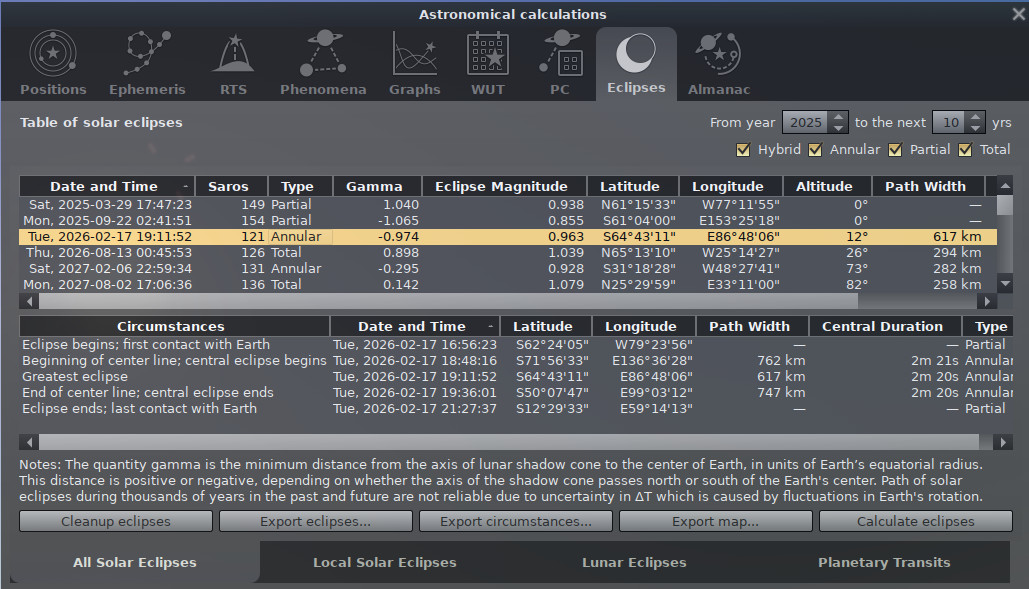
\includegraphics[width=0.8\textwidth]{astrocalc_dialog_eclipses_ase.jpg}
\caption{Astronomical Calculations (AstroCalc): Eclipses / All Solar Eclipses}
\label{fig:gui:AstroCalc:Eclipses:AllSolarEclipses}
\end{figure}

\noindent This subtab (Fig.~\ref{fig:gui:AstroCalc:Eclipses:AllSolarEclipses}) contains data for all solar eclipses on the Earth in the selected time range. 
Double click on a line in the table will set location and time of greatest eclipse. Click on the table row will show circumstances of selected eclipse in the lower table.

The quantity Gamma is the minimum distance of the lunar shadow cone axis to the center of the Earth, in units of Earth’s equatorial radius.
This distance is positive or negative, depending on whether the axis of the shadow cone passes north or south of the Earth's center.

Click the \menu{Export KML\ldots} button to create a KML file of the
selected eclipse. KML is a file format used to display geographic data
in Earth browsers, such as \program{Marble}, \program{Google Earth} or
\program{Google Maps}. The file can be opened in applications that
support KML version~2.2. A description of the lines for solar eclipses
is shown in Fig.~\ref{fig:gui:AstroCalc:Eclipses:EclipseMap}.
Different colors are used to draw path of central eclipse. Red = total
eclipse, blue = annular eclipse, and purple = hybrid eclipse. Limits
of penumbral or partial eclipse are green.

\begin{figure}[htbp]
\centering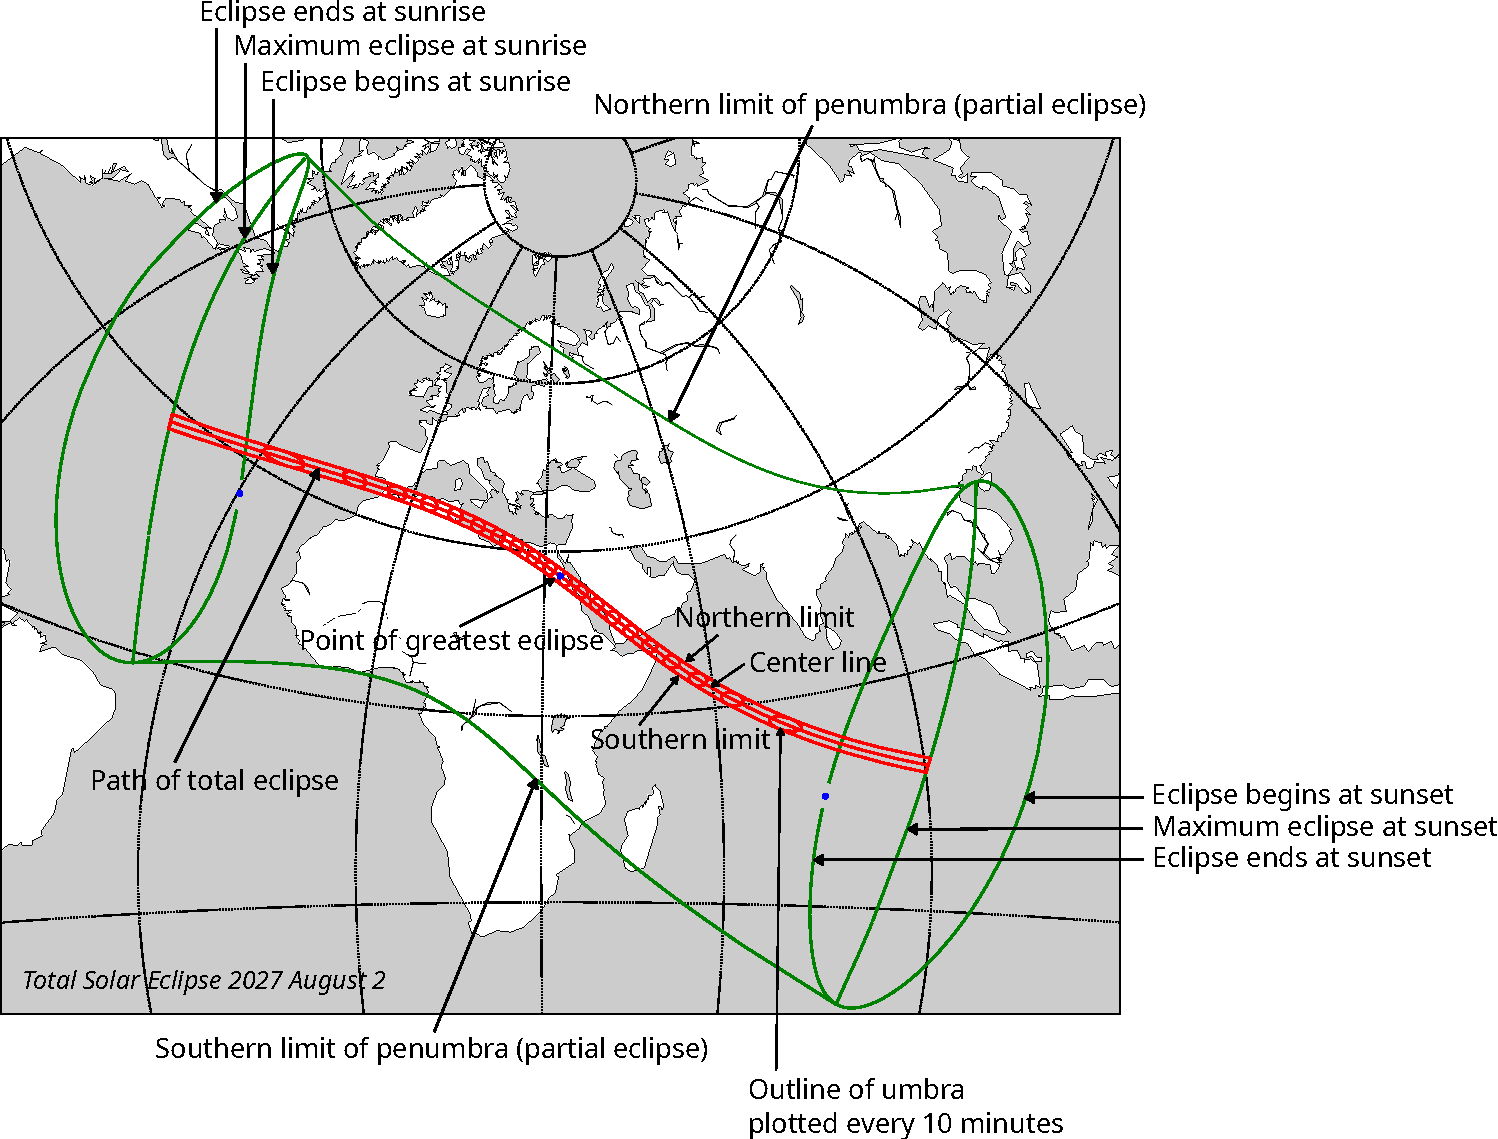
\includegraphics[width=0.95\textwidth]{eclipsemap.pdf}
\caption{Key to solar eclipse map}
\label{fig:gui:AstroCalc:Eclipses:EclipseMap}
\end{figure}

\subsubsection{The ``Local Solar Eclipses'' Subtab}
\label{sec:gui:AstroCalc:Eclipses:LocalSolarEclipses}

This subtab (Fig.~\ref{fig:gui:AstroCalc:Eclipses:LocalSolarEclipses}) contains data for solar eclipses for the current location (on the Earth!) in defined time range. 

Double click on a line in the table will set the time of greatest eclipse.

\begin{figure}[htbp]
\centering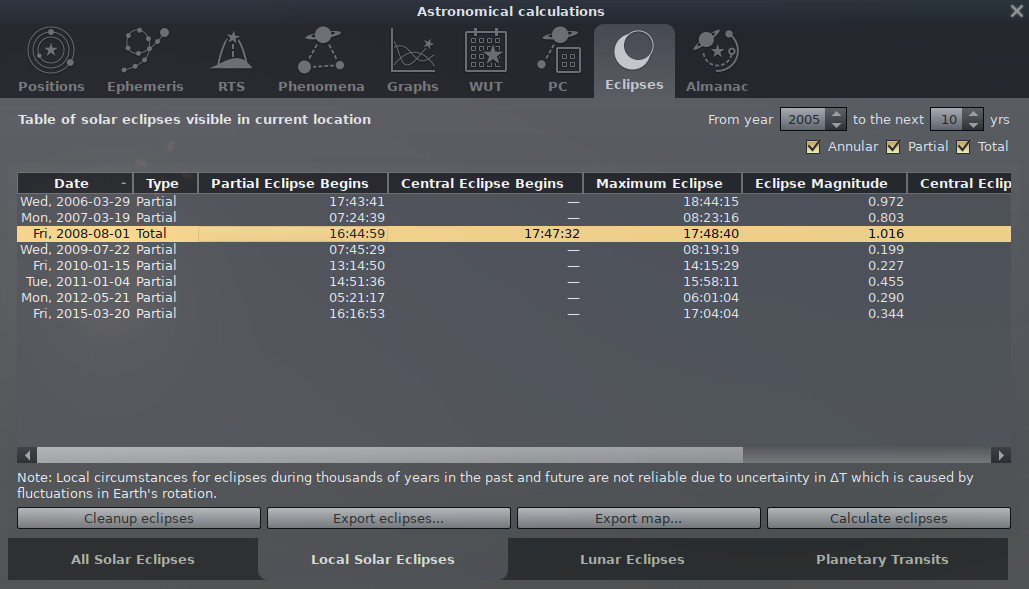
\includegraphics[width=0.8\textwidth]{astrocalc_dialog_eclipses_lse.jpg}
\caption{Astronomical Calculations (AstroCalc): Eclipses / Local Solar Eclipses}
\label{fig:gui:AstroCalc:Eclipses:LocalSolarEclipses}
\end{figure}


\subsubsection{The ``Lunar Eclipses'' Subtab}
\label{sec:gui:AstroCalc:Eclipses:LunarEclipses}

This subtab (Fig.~\ref{fig:gui:AstroCalc:Eclipses:LunarEclipses}) contains data for all lunar eclipses on the Earth in defined time range.
Double click on the table row will set time of greatest eclipse. Click on the table row will show circumstances of selected eclipse in the lower table.

The quantity gamma is the minimum distance from the center of the Moon to the axis of Earth’s umbral shadow cone, in units of Earth’s equatorial radius.
This distance is positive or negative, depending on whether the Moon passes north or south of the shadow cone axis.

\begin{figure}[p]
\centering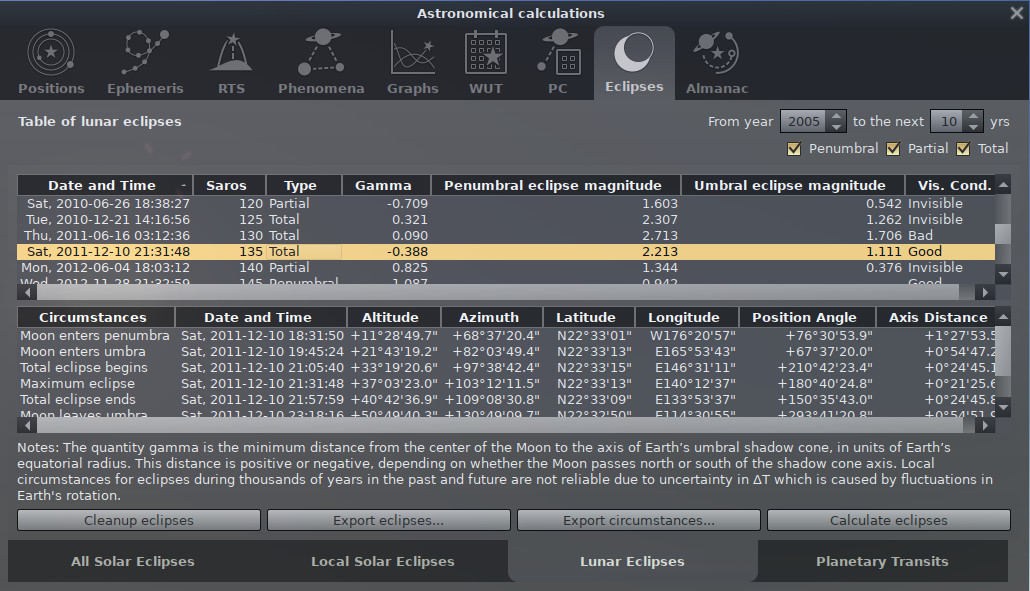
\includegraphics[width=0.8\textwidth]{astrocalc_dialog_eclipses_le.jpg}
\caption{Astronomical Calculations (AstroCalc): Eclipses / Lunar Eclipses}
\label{fig:gui:AstroCalc:Eclipses:LunarEclipses}
\end{figure}

The visibility conditions are based on the altitude of the Moon at greatest eclipse:
\begin{description}
  \item[Invisible] --- the greatest eclipse is invisible at the current location (altitude is negative);
  \item[Not obs.] --- not observable eclipse. Our rule of thumb is that a partial penumbral eclipse is detectable with the unaided eye if penumbral magnitude > 0.7;
  \item[Bad] --- bad visibility conditions for current location (altitude range is 0---30$\degree$);
  \item[Good] --- good visibility conditions for current location (altitude range is 30---45$\degree$; i.e., ``photometric altitude'');
  \item[Perfect] --- perfect visibility conditions for current location (altitude range is 45---90$\degree$).
\end{description}

\subsubsection{The ``Planetary Transits'' Subtab}\newFeature{0.22.2}
\label{sec:gui:AstroCalc:Eclipses:PlanetaryTransits}

This subtab (Fig.~\ref{fig:gui:AstroCalc:Eclipses:PlanetaryTransits})
contains data for all transits of Mercury and Venus across the Sun as
seen from Earth (see \ref{sec:Eclipses:Transits}) in the defined time
range.  If an event is not observable because the Sun/planet is below
the horizon, its time will be shown in brackets and
greyed-out. Further columns show the total duration of the event, and
the observable duration at the current location, which takes rising
and setting times into account.

Double click on the table row will set time of mid-transit.

\begin{figure}[htp]
\centering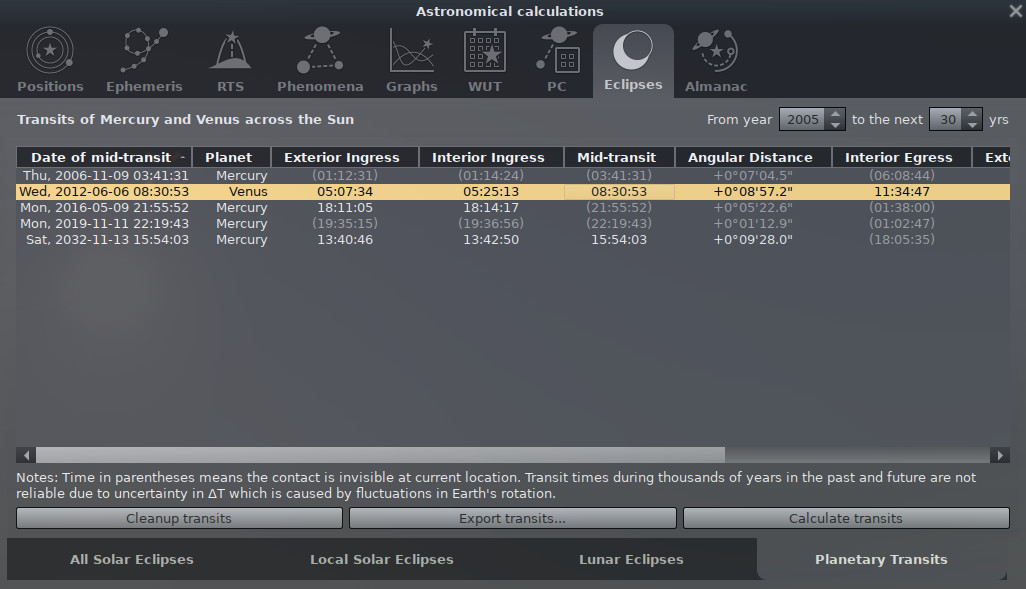
\includegraphics[width=0.8\textwidth]{astrocalc_dialog_transits.jpg}
\caption{Astronomical Calculations (AstroCalc): Eclipses / Planetary Transits}
\label{fig:gui:AstroCalc:Eclipses:PlanetaryTransits}
\end{figure}

\clearpage
\section{The Help Window}
\label{sec:gui:help}

\subsection{The Help Tab}
\label{sec:gui:help:help}
\begin{figure}[htp]
\centering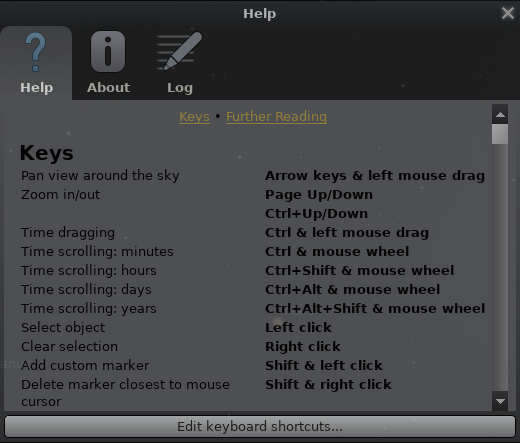
\includegraphics[width=0.51\textwidth]{help_dialog.png}
\caption{Help Window}
\label{fig:gui:help}
\end{figure}

\noindent The Help Tab lists all of Stellarium's keystrokes. Note that some
features are only available as keystrokes, so it's a good idea to have
a browse of the information in this window.

\subsection{The About Tab}
\label{sec:gui:help:about}
\begin{figure}[tbp]
\centering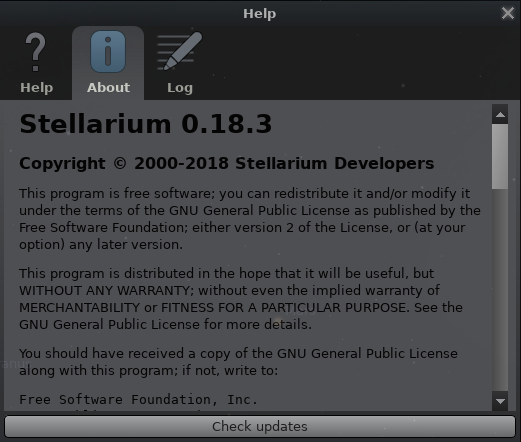
\includegraphics[width=0.51\textwidth]{help_dialog_about.png}
\caption{Help Window: About}
\label{fig:gui:help:about}
\end{figure}

The About Tab (Fig.~\ref{fig:gui:help:about}) shows version and licensing information, and a list of people who helped to produce the program.
This tab \newFeature{0.18.3} also provides a tool to check for updates of Stellarium.

\subsection{The Log Tab}
\label{sec:gui:help:log}
\begin{figure}[tbp]
\centering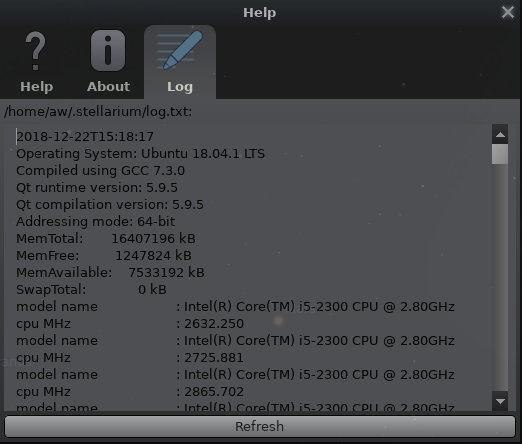
\includegraphics[width=0.51\textwidth]{help_dialog_log.png}
\caption{Help Window: Logfile}
\label{fig:gui:help:log}
\end{figure}

The Log Tab (Fig.~\ref{fig:gui:help:log}) shows messages like the loading confirmations carried out when
Stellarium runs. It is useful to locate the files that Stellarium writes
to your computer. The same information is written to  the file \file{log.txt} that you will
find in your user data directory (see~\ref{sec:Directories}).

\subsection{The Config Tab}
\label{sec:gui:help:config}
\begin{figure}[tbp]
	\centering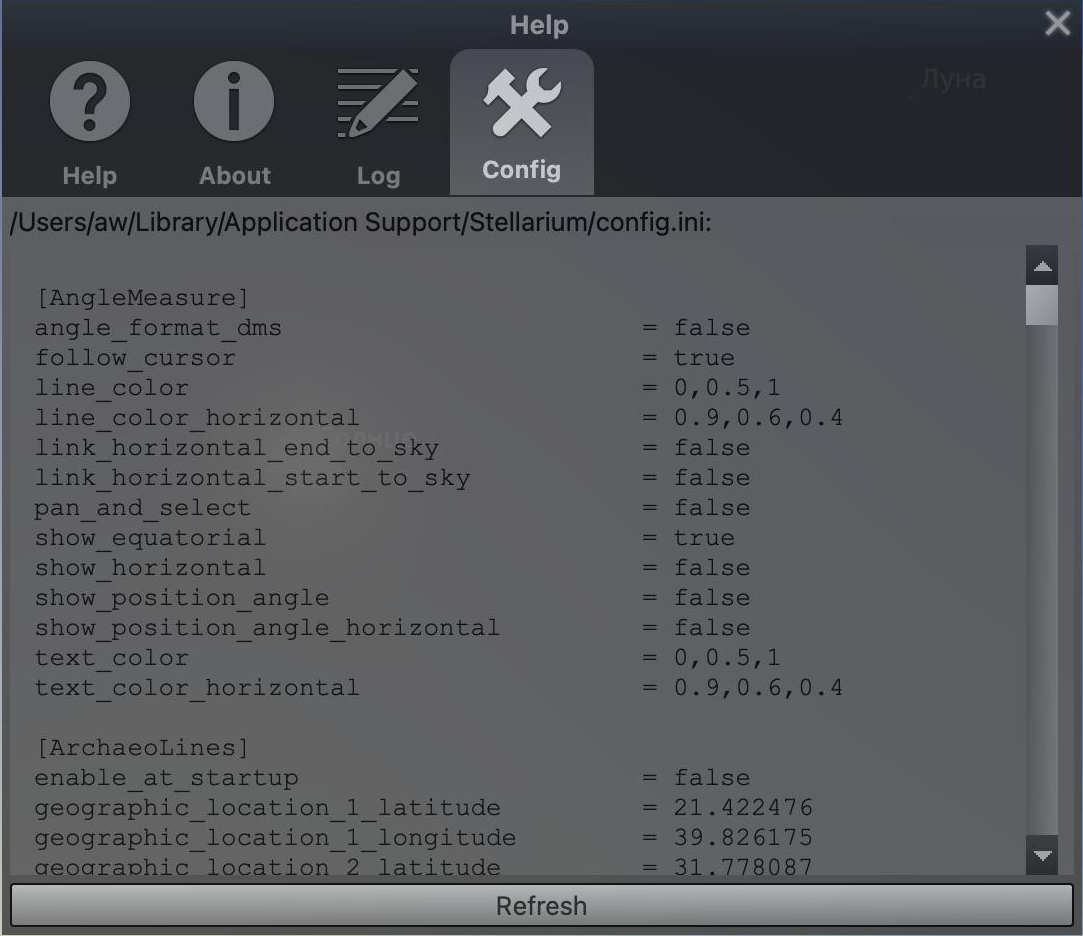
\includegraphics[width=0.51\textwidth]{help_dialog_config.png}
	\caption{Help Window: Config file}
	\label{fig:gui:help:config}
\end{figure}

The Config Tab (Fig.~\ref{fig:gui:help:config}) shows configuration data of the Stellarium. It is useful to locate the files that Stellarium writes
to your computer. The same information is written to  the file \file{config.ini} that you will
find in your user data directory (see~\ref{sec:Directories}).

\clearpage
\section{Editing Keyboard Shortcuts}
\label{sec:gui:help:hotkeys}

\begin{figure}[htbp]
\centering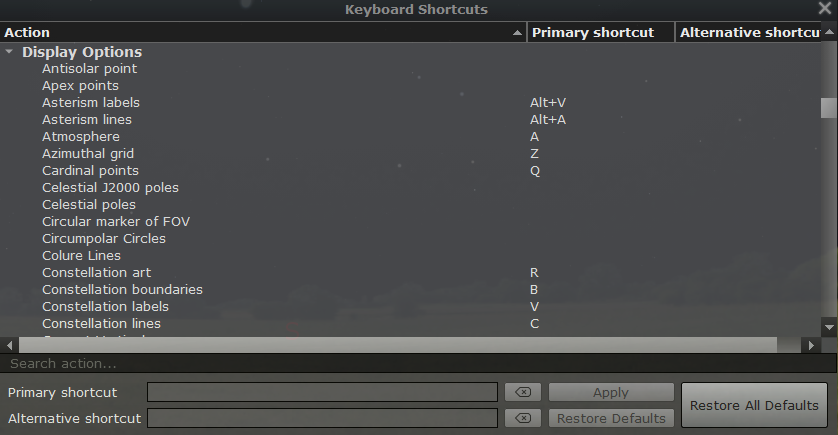
\includegraphics[width=0.8\textwidth]{hotkeys_dialog.png}
\caption{Keyboard Shortcuts}
\label{fig:gui:hotkeys}
\end{figure}

You can edit the shortcut keys here. Each available function can be
configured with up to two key combinations. You may want to
reconfigure keys for example if you have a non-English keyboard layout
and some keys either do not work at all, or feel unintuitive for you,
or if you are familiar with other software and want to use the same
hotkeys for similar functions. Simply select the function and click
with the mouse into the edit field, then press your key of choice. If
the key has been taken already, a message will tell you.

This tool is available through the Help Tab of the Help window (see section~\ref{sec:gui:help:help}) and the
Tools Tab of the Configuration window (see section~\ref{sec:gui:configuration:tools}).

\subsection{Example}
\label{sec:gui:help:hotkeys:example}

If you want \newFeature{0.21.2} to follow the sky view each evening
with the Sun at the same depth below the horizon, so that the twilight
is of equal darkness, you may want to assign some actions to intuitive
shortcut keys. In the Keyboard Shortcut editor
(Fig.~\ref{fig:gui:hotkeys}), find the \emph{Date and Time} group and
assign, e.g., the keys on your numeric keypad:

\begin{tabular}{ll}
  Previous evening twilight & Ctrl+9 \\
  Previous morning twilight & Ctrl+7 \\
  Next evening twilight     & Ctrl+3 \\
  Next morning twilight     & Ctrl+1 \\
  Today's evening twilight  & Ctrl+6 \\
  Today's morning twilight  & Ctrl+4 \\
\end{tabular}









%%% Local Variables: 
%%% mode: latex
%%% TeX-master: "guide"
%%% End: 
